\documentclass[10pt,a4paper,titlepage,parskip]{scrartcl}
\usepackage[utf8]{inputenc}
\usepackage{pdfpages}
\usepackage[english]{babel}
\renewcommand\familydefault{\sfdefault}
\usepackage{color}
\usepackage{etoolbox}
\usepackage{lastpage}
\usepackage{hyperref}
\usepackage{framed}
\usepackage{subcaption}
\usepackage{enumerate}
\usepackage{amssymb}

% adjust the page margins
\usepackage[left=2.5cm,right=2.5cm,top=2.5cm,bottom=3.0cm]{geometry}

\usepackage{fancyhdr}
\pagestyle{fancy}

\definecolor{myBlue}{rgb}{0.2,0.4,0.65}
\definecolor{ufzgray1}{RGB}{81,81,81}
\definecolor{ufzgray2}{RGB}{156,156,156}
\definecolor{ufzgray3}{RGB}{185,185,185}

\patchcmd{\headrule}{\hrule}{\color{myBlue}\hrule}{}{}
\patchcmd{\footrule}{\hrule}{\color{myBlue}\hrule}{}{}

% dots after section numbers
\renewcommand{\thesection}{\arabic{section}.}
\renewcommand{\thesubsection}{\arabic{section}.\arabic{subsection}.}

% make an entire region tt font
\newenvironment{ttfont}{\fontfamily{\ttdefault}\selectfont}{\par}

% My style
\usepackage{xcolor}
\definecolor{jmcolor}{RGB}{255,127,0}
\newcommand{\jm}[1]{\textcolor{jmcolor}{#1}}
\newcommand{\jmout}[1]{\textcolor{jmcolor}{\sout{#1}}}
\newcommand{\GRAU}[1]{\textcolor{ufzgray2}{#1}}

%\newcommand{\footrulecolor}{myBlue}
\rhead{}
\lhead{}
\chead{\textcolor{myBlue}{\footnotesize Project Documentation ``Improving characterization of flood-producing precipitation events in HFE database''}}
\lfoot{\textcolor{myBlue}{\footnotesize Telephone: +1 (226) 505-5600}}
\cfoot{\textcolor{myBlue}{\footnotesize e-mail: juliane.mai@uwaterloo.ca}}
\rfoot{\textcolor{myBlue}{\footnotesize Page \thepage \ of \pageref{LastPage}}}
\renewcommand{\footrulewidth}{0.4pt} 

% Hurenkinder und Schusterjungen verhindern
\clubpenalty10000
\widowpenalty10000
\displaywidowpenalty=10000

\includepdfset{pages=-}

% colored lines
\makeatletter
\let\old@rule\@rule
\def\@rule[#1]#2#3{\textcolor{rulecolor}{\old@rule[#1]{#2}{#3}}}
\makeatother

% fixed width columns in table
\usepackage{array}
\newcolumntype{L}[1]{>{\raggedright\let\newline\\\arraybackslash\hspace{0pt}}p{#1}}
\newcolumntype{C}[1]{>{\centering\let\newline\\\arraybackslash\hspace{0pt}}p{#1}}
\newcolumntype{R}[1]{>{\raggedleft\let\newline\\\arraybackslash\hspace{0pt}}p{#1}}

%\linespread{1.5}

\begin{document}  
	
	\vspace*{-1cm}
	\pagestyle{fancy}
	
	\begin{center}
		Juliane Mai, Ph.D.\\
		Technical Consulting\\[4pt]
		405-460A Belmont Ave W., \\
		Kitchener, ON, N2M 0A9, Canada\\[10pt]
		{\definecolor{rulecolor}{named}{myBlue}\rule{\linewidth}{0.4pt}}
	\end{center}
	\begin{center}
		\textcolor{myBlue}{{\Large --~Documentation~--}}\\[4pt]
		Improving the characterization of the flood-producing precipitation events in the Historic Flood Event (HFE) database by using the CaPA reanalysis/analysis\\[4pt]
	\end{center}
	
\tableofcontents
\pagebreak

\section{Meetings}

\subsection{Kick-off meeting}
\vspace*{-0.5cm}
\begin{tabbing}
	\hspace{2.8cm} \= \hspace{4cm} \= \kill \\
	\textbf{Date and time:} 	\> Aug 25, 2022 1-2pm\\
	\textbf{Attendees:} 	\> Dikra Khedhaouiria \> (dikraa.khedhaouiria@ec.gc.ca)\\
							\> Juliane Mai \> (juliane.mai@uwaterloo.ca)\\
							\> Marie-Eve Martin \> (marie-eve.martin@nrcan-rncan.gc.ca)\\
							\> Philippe Aussant \> (philippe.aussant@NRCan-RNCan.gc.ca)\\
	                        \> Pierre-Etienne Bonhomme \> (etienne.bonhomme@NRCan-RNCan.gc.ca)\\
	                        \> Vincent Fortin \> (vincent.fortin@ec.gc.ca)
\end{tabbing}
\vspace*{-0.5cm}
\textbf{Notes:}
\begin{itemize}
	\setlength\itemsep{-0.8em}
	\item discussion of access to resources (HFE database, Geomet requests, CaSPAr requests)
	\item discussion of formats (JSON, PNG, i.e., mimicking formats that are received when requesting data from GeoMet)
	\item discussion of handling liquid/solid precipitation (Vincent suggested manuscript in preparation that will require humidity and temperature as additional variables to transform precipitation into components)
	\item next meeting mid September will be scheduled by Dikra
\end{itemize}

\subsection{Mid-contract follow-up meeting}
\vspace*{-0.5cm}
\begin{tabbing}
	\hspace{2.8cm} \= \hspace{4cm} \= \kill \\
	\textbf{Date and time:} 	\> Sep 15, 2022 2-3pm\\
	\textbf{Attendees:} 	\> Catherine Vachon \> (catherine.vachon@NRCan-RNCan.gc.ca)\\
	\> Dikra Khedhaouiria \> (dikraa.khedhaouiria@ec.gc.ca)\\
	\> Juliane Mai \> (juliane.mai@uwaterloo.ca)\\
	\> Milena Dimitrijevic \> (milena.dimitrijevic@ec.gc.ca)\\
	%\> Marie-Eve Martin \> (marie-eve.martin@nrcan-rncan.gc.ca)\\
	\> Philippe Aussant \> (philippe.aussant@NRCan-RNCan.gc.ca)\\
	%\> Pierre-Etienne Bonhomme \> (etienne.bonhomme@NRCan-RNCan.gc.ca)\\
	\> Vincent Fortin \> (vincent.fortin@ec.gc.ca)
\end{tabbing}
\vspace*{-0.5cm}
\textbf{Notes:}
\begin{itemize}
\setlength\itemsep{-0.8em}
\item presentation of functions/modules implemented so far (a1-a3,b1-b3,cx,dx,ex,fx)
\item discussion of missing files on GeoMet
\item discussion of how to proceed with ``training'': sharing GitHub as is with Philippe and Catherine such that they can start testing setup of Python environment and functions
\end{itemize}

%\section{Resources}
%
%\begin{itemize}
%	\setlength\itemsep{-0.8em}
%	\item access to the HFE database:\\
%	\url{https://open.canada.ca/data/en/dataset/fe83a604-aa5a-4e46-903c-685f8b0cc33c}
%	\item query to obtain RDPA 24h total precipitation for a 1x1 degree box centered on Montreal:\\
%	\url{https://api.weather.gc.ca/collections/weather:rdpa:10km:24f/coverage?f=json&datetime=2017-05-12T12Z&CRS=EPSG:4326&bbox=-74,45,-73,46}
%	\item documentation of requests from GeoMet:\\
%	\url{https://eccc-msc.github.io/open-data/msc-geomet/web-services_en/}\\
%	see specifically OGC API:\\
%	\url{https://eccc-msc.github.io/open-data/msc-geomet/web-services_en/#ogc-api-features}
%\end{itemize}
\pagebreak

\section{Request, read, and plot data from GeoMet}

The assumption is that we want to retrieve CaPA data (RDPA; 24h total precipitation) from GeoMet for Aug 9, 2018 around Montreal ($\mathrm{lat} = 45.5019^{\circ}\mathrm{N}$, $\mathrm{lon}=-73.5674^{\circ}\mathrm{E}$). 

The URL to request is the following:
\url{https://api.weather.gc.ca/collections/weather:rdpa:10km:24f/coverage?f=json&datetime=2022-08-24T12Z&CRS=EPSG:4326&bbox=-74,45,-73,46}

This returns the following JSON string (not geo-referenced):
\begin{framed}	
		\texttt{\{"type": "Coverage", "domain": \{"type": "Domain", "domainType": "Grid", "axes": \{"x": \{"start": -74.0, "stop": -73.0, "num": 15\}, "y": \{"start": 46.0, "stop": 45.0, "num": 16\}\}, "referencing": [\{"coordinates": ["x", "y"], "system": \{"type": "GeographicCRS", "id": "http://www.opengis.net/def/crs/OGC/1.3/CRS84"\}\}]\}, "parameters": \{"APCP": \{"type": "Parameter", "description": "Total precipitation [kg/(m\^{}2)]", "unit": \{"symbol": "[kg/(m\^{}2)]"\}, "observedProperty": \{"id": "0-SFC", "label": \{"en": "Total precipitation [kg/(m\^{}2)]"\}\}\}\}, "ranges": \{"APCP": \{"type": "NdArray", "dataType": "float", "axisNames": ["y", "x"], "shape": [16, 15], "values": [null, null, null, null, null, null, null, null, null, null, null, null, null, null, null, null, null, null, null, null, null, 9.300250053405762, 12.344250679016113, null, null, null, null, null, null, null, null, null, null, null, null, 5.607500076293945, 9.330750465393066, 13.382000923156738, 16.639751434326172, null, null, null, null, null, null, $\ldots$ , null, null, null, null, null, null, null, 10.574250221252441, 11.665250778198242, 11.032000541687012, null, null, null, null, null, null, null, null, null, null, null, null, 9.582500457763672, 10.17750072479248, null, null, null, null, null, null, null, null, null, null, null, null, null, null, null, null, null, null, null, null, null]\}\}\}}\\
\end{framed}

This corresponds to the following 2D view of the data (not geo-referenced):
\begin{table}[h]
	\begin{tabular}{R{0.5cm}R{0.5cm}R{0.5cm}R{0.5cm}R{0.5cm}R{0.5cm}R{0.5cm}R{0.5cm}R{0.5cm}R{0.5cm}R{0.5cm}R{0.5cm}R{0.5cm}R{0.5cm}R{0.5cm}}
- & - & - & - & - & - & - & - & - & - & - & - & - & - & -\\
- & - & - & - & - & - & 9 & 12 & - & - & - & - & - & - & -\\
- & - & - & - & - & 6 & 9 & 13 & 17 & - & - & - & - & - & -\\
- & - & - & - & 4 & 6 & 9 & 13 & 17 & 21 & - & - & - & - & -\\
- & - & 3 & 3 & 4 & 6 & 11 & 16 & 19 & 22 & - & - & - & - & -\\
- & 4 & 3 & 3 & 3 & 6 & 13 & 18 & 22 & 25 & 23 & - & - & - & -\\
- & 5 & 4 & 3 & 3 & 5 & 12 & 19 & 23 & 28 & 26 & 28 & - & - & -\\
- & - & 5 & 3 & 2 & 4 & 12 & 18 & 23 & 26 & 27 & 32 & 38 & - & -\\
- & - & - & 3 & 2 & 4 & 10 & 16 & 20 & 22 & 26 & 35 & 38 & 27 & -\\
- & - & - & - & 4 & 5 & 8 & 16 & 18 & 20 & 27 & 36 & 35 & 24 & -\\
- & - & - & - & 6 & 6 & 7 & 14 & 16 & 20 & 31 & 41 & 35 & 20 & -\\
- & - & - & - & - & 5 & 8 & 11 & 13 & 16 & 27 & 37 & 33 & - & -\\
- & - & - & - & - & - & 10 & 10 & 12 & 11 & 19 & 26 & - & - & -\\
- & - & - & - & - & - & - & 11 & 12 & 11 & - & - & - & - & -\\
- & - & - & - & - & - & - & 10 & 10 & - & - & - & - & - & -\\
- & - & - & - & - & - & - & - & - & - & - & - & - & - & -\\				
	\end{tabular}
\end{table}
\pagebreak

To retrieve the corresponding PNG file for this data use (see Fig.~\ref{fig:plot_example:geo-weather}) (not geo-referenced):
\begin{framed}
\url{https://geo.weather.gc.ca/geomet?SERVICE=WMS&VERSION=1.3.0&REQUEST=GetMap&LAYERS=RDPA.24F_PR&STYLES=RDPA-WXO&CRS=EPSG:4326&BBOX=45,-74,46,-73&WIDTH=400&HEIGHT=400&FORMAT=image/png&TIME=2022-08-24T12:00:00Z&DIM_REFERENCE_TIME=2022-08-24T12:00:00Z}
\end{framed}
To retrieve the legend use (see Fig.~\ref{fig:plot_example:geo-weather}):
\begin{framed}
	\url{https://geo.weather.gc.ca/geomet?SERVICE=WMS&VERSION=1.3.0&REQUEST=GetLegendGraphic&LAYERS=RDPA.24F_PR&STYLES=RDPA-WXO&CRS=EPSG:4326&BBOX=45,-74,46,-73&WIDTH=400&HEIGHT=400&FORMAT=image/png&TIME=2022-08-24T12:00:00Z&DIM_REFERENCE_TIME=2022-08-24T12:00:00Z}
\end{framed}

To actually retrieve the geo-referenced data used for those plots, the GRIB2 file needs to be retrieved using the following command:
\begin{framed}
\texttt{\url{https://api.weather.gc.ca/collections/weather:rdpa:10km:24f/coverage?f=GRIB&datetime=2022-08-24T12Z&CRS=EPSG:4326&bbox=-74,45,-73,46}}
\end{framed}
This seems to be the only possibility to obtain geo-referenced data. The library developed here now provides three functions to obtain and plot the data. The results are shown in Fig.~\ref{fig:plot_example:api-weather}.

\textbf{Step A1:} Request data using the Geomet API (\url{https://api.weather.gc.ca}).
\begin{framed}
	\vspace*{-1.2cm}
	\begin{ttfont}
	\begin{tabbing}
		\hspace{1.0cm} \= \hspace{3.9cm} \= \kill \\[4pt]
		\GRAU{\# see module for detailed documentation and example}\\
		from a1\_request\_geomet\_grib2 import request\_geomet\_grib2\\
		\\
		files\_geomet = request\_geomet\_grib2(\\
		\> \GRAU{\# Mandatory arguments:}\\
		\> product=\textit{product}, \> \GRAU{\# name of product, e.g., "rdpa:10km:24f"}\\
		\> date=\textit{date},\> \GRAU{\# datetime object specifying date (or list of dates)}\\
		\> bbox=\textit{bbox},\> \GRAU{\# dictionary specifying bounding box}\\
		\> \GRAU{\# Optional arguments:}\\
		\> crs=\textit{crs},\> \GRAU{\# coordinate reference system, e.g., "EPSG:4326"}\\
		\> filename=\textit{filename},\> \GRAU{\# base filename of output file (can include path but }\\
		\>                           \> \GRAU{\# no file extension); date will be added to filename}\\
		\> overwrite=\textit{overwrite},\> \GRAU{\# If true, file will be downloaded }\\
		\>                           \> \GRAU{\# again overwriting existing file}\\
		\> silent=\textit{silent}, \> \GRAU{\# True for no printing on screen}\\
		\> ) \> 
	\end{tabbing}
	\end{ttfont}
	\vspace*{-0.3cm}
\end{framed}
\vspace*{-0.3cm}
The return variable \texttt{files\_geomet} is a dictionary where the keys are the provides date(s) and the values are lists of filenames that contain this time step. If the file already existed, it will not be overwritten unless \texttt{overwrite} is set to \texttt{True}. The filename will be returned nonetheless. In case no file is found for a date, the list will be empty. If the list contains multiple files, the time step was found in several files. If no file was found for any date, an error is raised since this indicates that something in the request string to Geomet is likely wrong. 
\pagebreak

\textbf{Step B1:} Read data from files requested.
\begin{framed}
	\vspace*{-1.2cm}
	\begin{ttfont}
		\begin{tabbing}
			\hspace{1.0cm} \= \hspace{5.2cm} \= \kill \\[4pt]
			\GRAU{\# see module for detailed documentation and example}\\
			from b1\_read\_geomet\_grib2 import read\_geomet\_grib2\\
			\\
			data\_geomet = read\_geomet\_grib2(\\
			\> \GRAU{\# Mandatory arguments:}\\
			\> filenames=\textit{filenames}, \> \GRAU{\# dictionary specifying filename per time}\\
			\>  \> \GRAU{\# step, e.g.,}\\
			\>  \> \GRAU{\#  \{ date\_1: [ filename\_1, filename\_2 ],}\\
			\>  \> \GRAU{\# \hspace*{0.2cm}    date\_2: [ filename\_2 ],}\\
			\>  \> \GRAU{\# \hspace*{0.2cm}    date\_3: [ ], ... \}}\\
			\>  \> \GRAU{\# $\curvearrowright$ output of "request\_geomet\_grib2()"}\\
			\> \GRAU{\# Optional arguments:}\\
			\> lintransform=\textit{lintransform}, \> \GRAU{\# dictionary to specify linear transform of}\\
			\>  \> \GRAU{\# data, e.g., to allow for unit conversions}\\
			\> silent=\textit{silent}, \> \GRAU{\# True for no printing on screen}\\
			\> ) \> 
		\end{tabbing}
	\end{ttfont}
	\vspace*{-0.3cm}
\end{framed}
\vspace*{-0.3cm}
The returned variable \texttt{data\_geomet} is a dictionary that will contain the attributes \texttt{time}, \texttt{lat}, \texttt{lon}, and \texttt{var}. The latter will be 3-dimensional (time, lat, lon). The latitude and longitudes of the files are checked for consistency. The time steps returned are only the time steps where data was available.

\textbf{Step Cx:} Plot data.
\begin{framed}
	\vspace*{-1.2cm}
	\begin{ttfont}
		\begin{tabbing}
			\hspace{1.0cm} \= \hspace{5.2cm} \= \kill \\[4pt]
			\GRAU{\# see module for detailed documentation and example}\\
			from cx\_plot\_data import plot\_data\\
			\\
			plot\_geomet = plot\_data(\\
			\> \GRAU{\# Mandatory arguments:}\\
			\> var=\textit{var}, \> \GRAU{\# 2D/3D array of values for variable}\\
			\> lat=\textit{lat}, \> \GRAU{\# 2D array of latitudes}\\
			\> lon=\textit{lon}, \> \GRAU{\# 2D array of longitudes}\\
			\> date=\textit{date}, \> \GRAU{\# date or list of dates as datetime objects}\\
			\> \GRAU{\# Optional arguments:}\\
			\> png=\textit{png}, \> \GRAU{\# True if PNG file(s) should be created}\\
			\> gif=\textit{gif}, \> \GRAU{\# True if GIF should be created}\\
			\> legend=\textit{legend}, \> \GRAU{\# True if PNG of legend should be created}\\
			\> cities=\textit{cities}, \> \GRAU{\# True to display cities on maps}\\
			\> bbox=\textit{bbox}, \> \GRAU{\# Bounding box will be plotted if provided}\\
			\> basefilename=\textit{basefilename}, \> \GRAU{\# String specifying basename of files created}\\
			\> overwrite=\textit{overwrite}, \> \GRAU{\# True to overwrite existing plots}\\
			\> silent=\textit{silent}, \> \GRAU{\# True for no printing on screen}\\
			\> ) \> 
		\end{tabbing}
	\end{ttfont}
	\vspace*{-0.3cm}
\end{framed}
\vspace*{-0.3cm}
The returned variable \texttt{plot\_geomet} is a dictionary that will contain the attributes \texttt{png}, \texttt{gif}, and \texttt{legend}. Each of them are assigned list of the according files created. If no file was created (e.g., no legend), the respective list will be empty.

\begin{figure}[h]
	\begin{subfigure}[b]{0.45\textwidth}
		\centering
		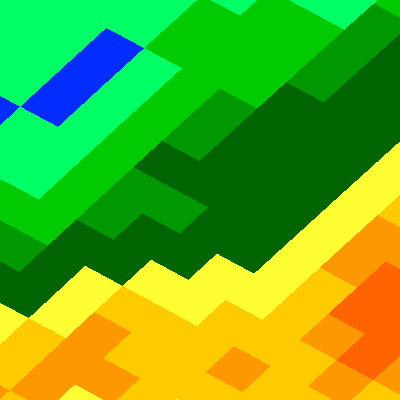
\includegraphics[height=0.58\linewidth]{figures/test-map-geomet-geo-weather-rdpa24_2018080912.png}
		\hspace*{0.5cm}
		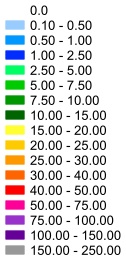
\includegraphics[height=0.58\linewidth]{figures/test-map-geomet-geo-weather-rdpa24_legend.png}
		\caption{Raw PNG and legend for RDPA-24h data retrieved using \url{https://geo.weather.gc.ca}\\(only displayed for reference)}
		\label{fig:plot_example:geo-weather}
	\end{subfigure}
	\hspace*{0.05\textwidth}
	\begin{subfigure}[b]{0.45\textwidth}
		\centering
		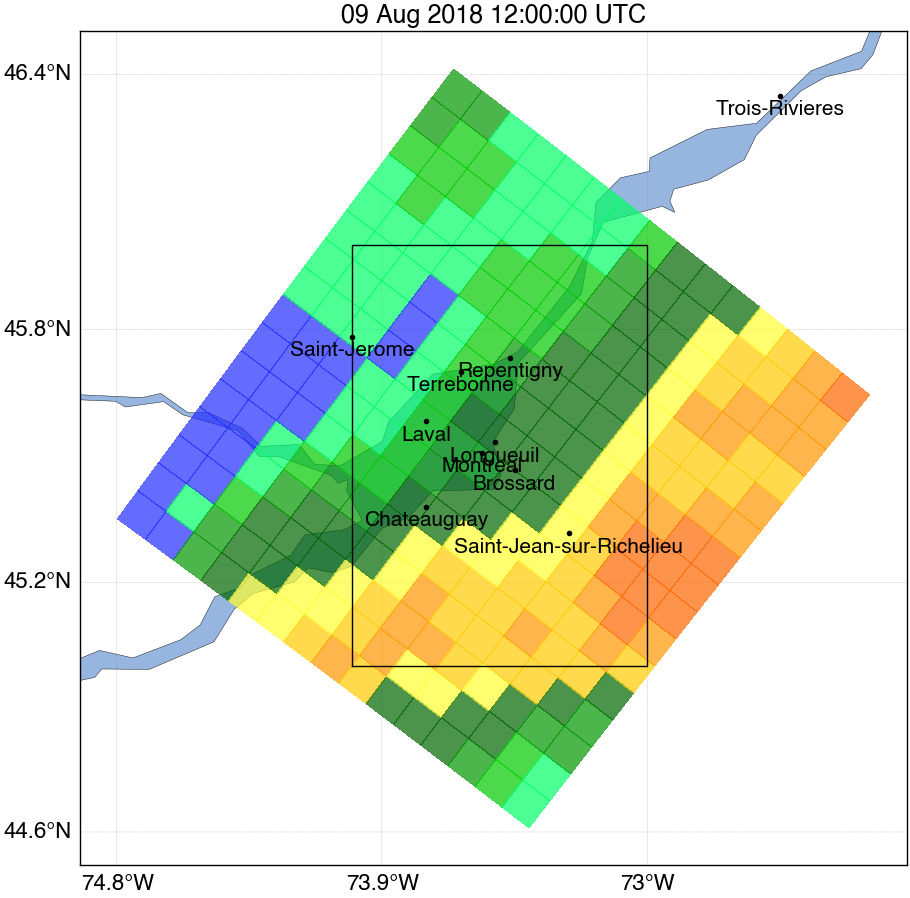
\includegraphics[height=0.58\linewidth]{figures/test-map-geomet-nrcan-hfe-rdpa24_2018080912.png}
		\hspace*{0.5cm}
		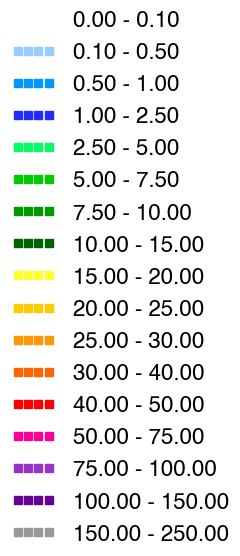
\includegraphics[height=0.58\linewidth]{figures/test-map-geomet-nrcan-hfe-rdpa24_legend.png}
		\caption{PNG and legend produced using NRCan-HFE library based on GRIB2 data (RDPA-24h) retrieved using \url{https://api.weather.gc.ca/}}
		\label{fig:plot_example:api-weather}
	\end{subfigure}
	\caption{RDPA (24h total precipitation) on Aug 9, 2018 (noon UTC) around Montreal}
	\label{fig:plot_example_geomet-api_vs_geomet-nrcan-hfe}
\end{figure}

\pagebreak

\section{Request, read, and plot data from CaSPAr}

\textbf{Step A2:} Request data using CaSPAr (\url{https://caspar-data.ca/caspar}).

The following function is just a dummy to provide some information on how to retrieve data from CaSPAr manually. Fig.~\ref{fig:request_data_caspar} shows the setting used to retrieve RDRS-v2.1 data from CaSPAr. The shapefile containing the domain of the HFE database is provided under \texttt{data/caspar/RDRS\_v21\_hfe\_outline.zip} (see shape as blue polygon in Fig.~\ref{fig:plot_example:location_points}). Some example data are made available (see \texttt{src/test-data/*.nc}). See more information on how to create a CaSPAr account, request and dwonload data under \url{https://github.com/julemai/CaSPAr/wiki/How-to-get-started-and-download-your-first-data}.

This function basically only checks if the files for the product specified and the (list of)
date(s) provided are available under the specified foldername.
\begin{framed}
	\vspace*{-1.2cm}
	\begin{ttfont}
		\begin{tabbing}
			\hspace{1.0cm} \= \hspace{4.1cm} \= \kill \\[4pt]
			\GRAU{\# see module for detailed documentation and example}\\
			from a2\_request\_caspar\_nc import request\_caspar\_nc\\
			\\
			files\_caspar = request\_caspar\_nc( \\
				\> \GRAU{\# Mandatory arguments:}\\
				\> product=\textit{product}, \> \GRAU{\# name of product in CaSPAr (e.g., 'RDRS-v2.1')} \\
				\> variable=\textit{variable}, \> \GRAU{\# name of variable in CaSPAr}\\
				\> \> \GRAU{\#  (e.g., 'RDRS\_v2.1\_A\_PR0\_SFC')}\\
				\> date=\textit{date}, \> \GRAU{\# datetime object specifying date}\\
				\> \> \GRAU{\#  (can be list of dates)}\\
				\> \GRAU{\# Optional arguments:}\\
				\> foldername=\textit{foldername}, \> \GRAU{\# } \\
				\> silent=\textit{silent}, \> \GRAU{\# True for no printing on screen} \\
			\> ) \> 
		\end{tabbing}
	\end{ttfont}
	\vspace*{-0.3cm}
\end{framed}
\vspace*{-0.3cm}
The return variable \texttt{files\_caspar} is a dictionary where the keys are the provides date(s) and the values are lists of filenames that contain this time step. In case no file is found for a date, the list will be empty. If the list contains multiple files, the time step was found in several files. If no file was found for any date, an error is raised since this indicates that the files have not been requested and downloaded from CaSPAr yet or the \texttt{foldername} is not the location where those files have been downloaded to. 
\begin{figure}[h]
	\centering
	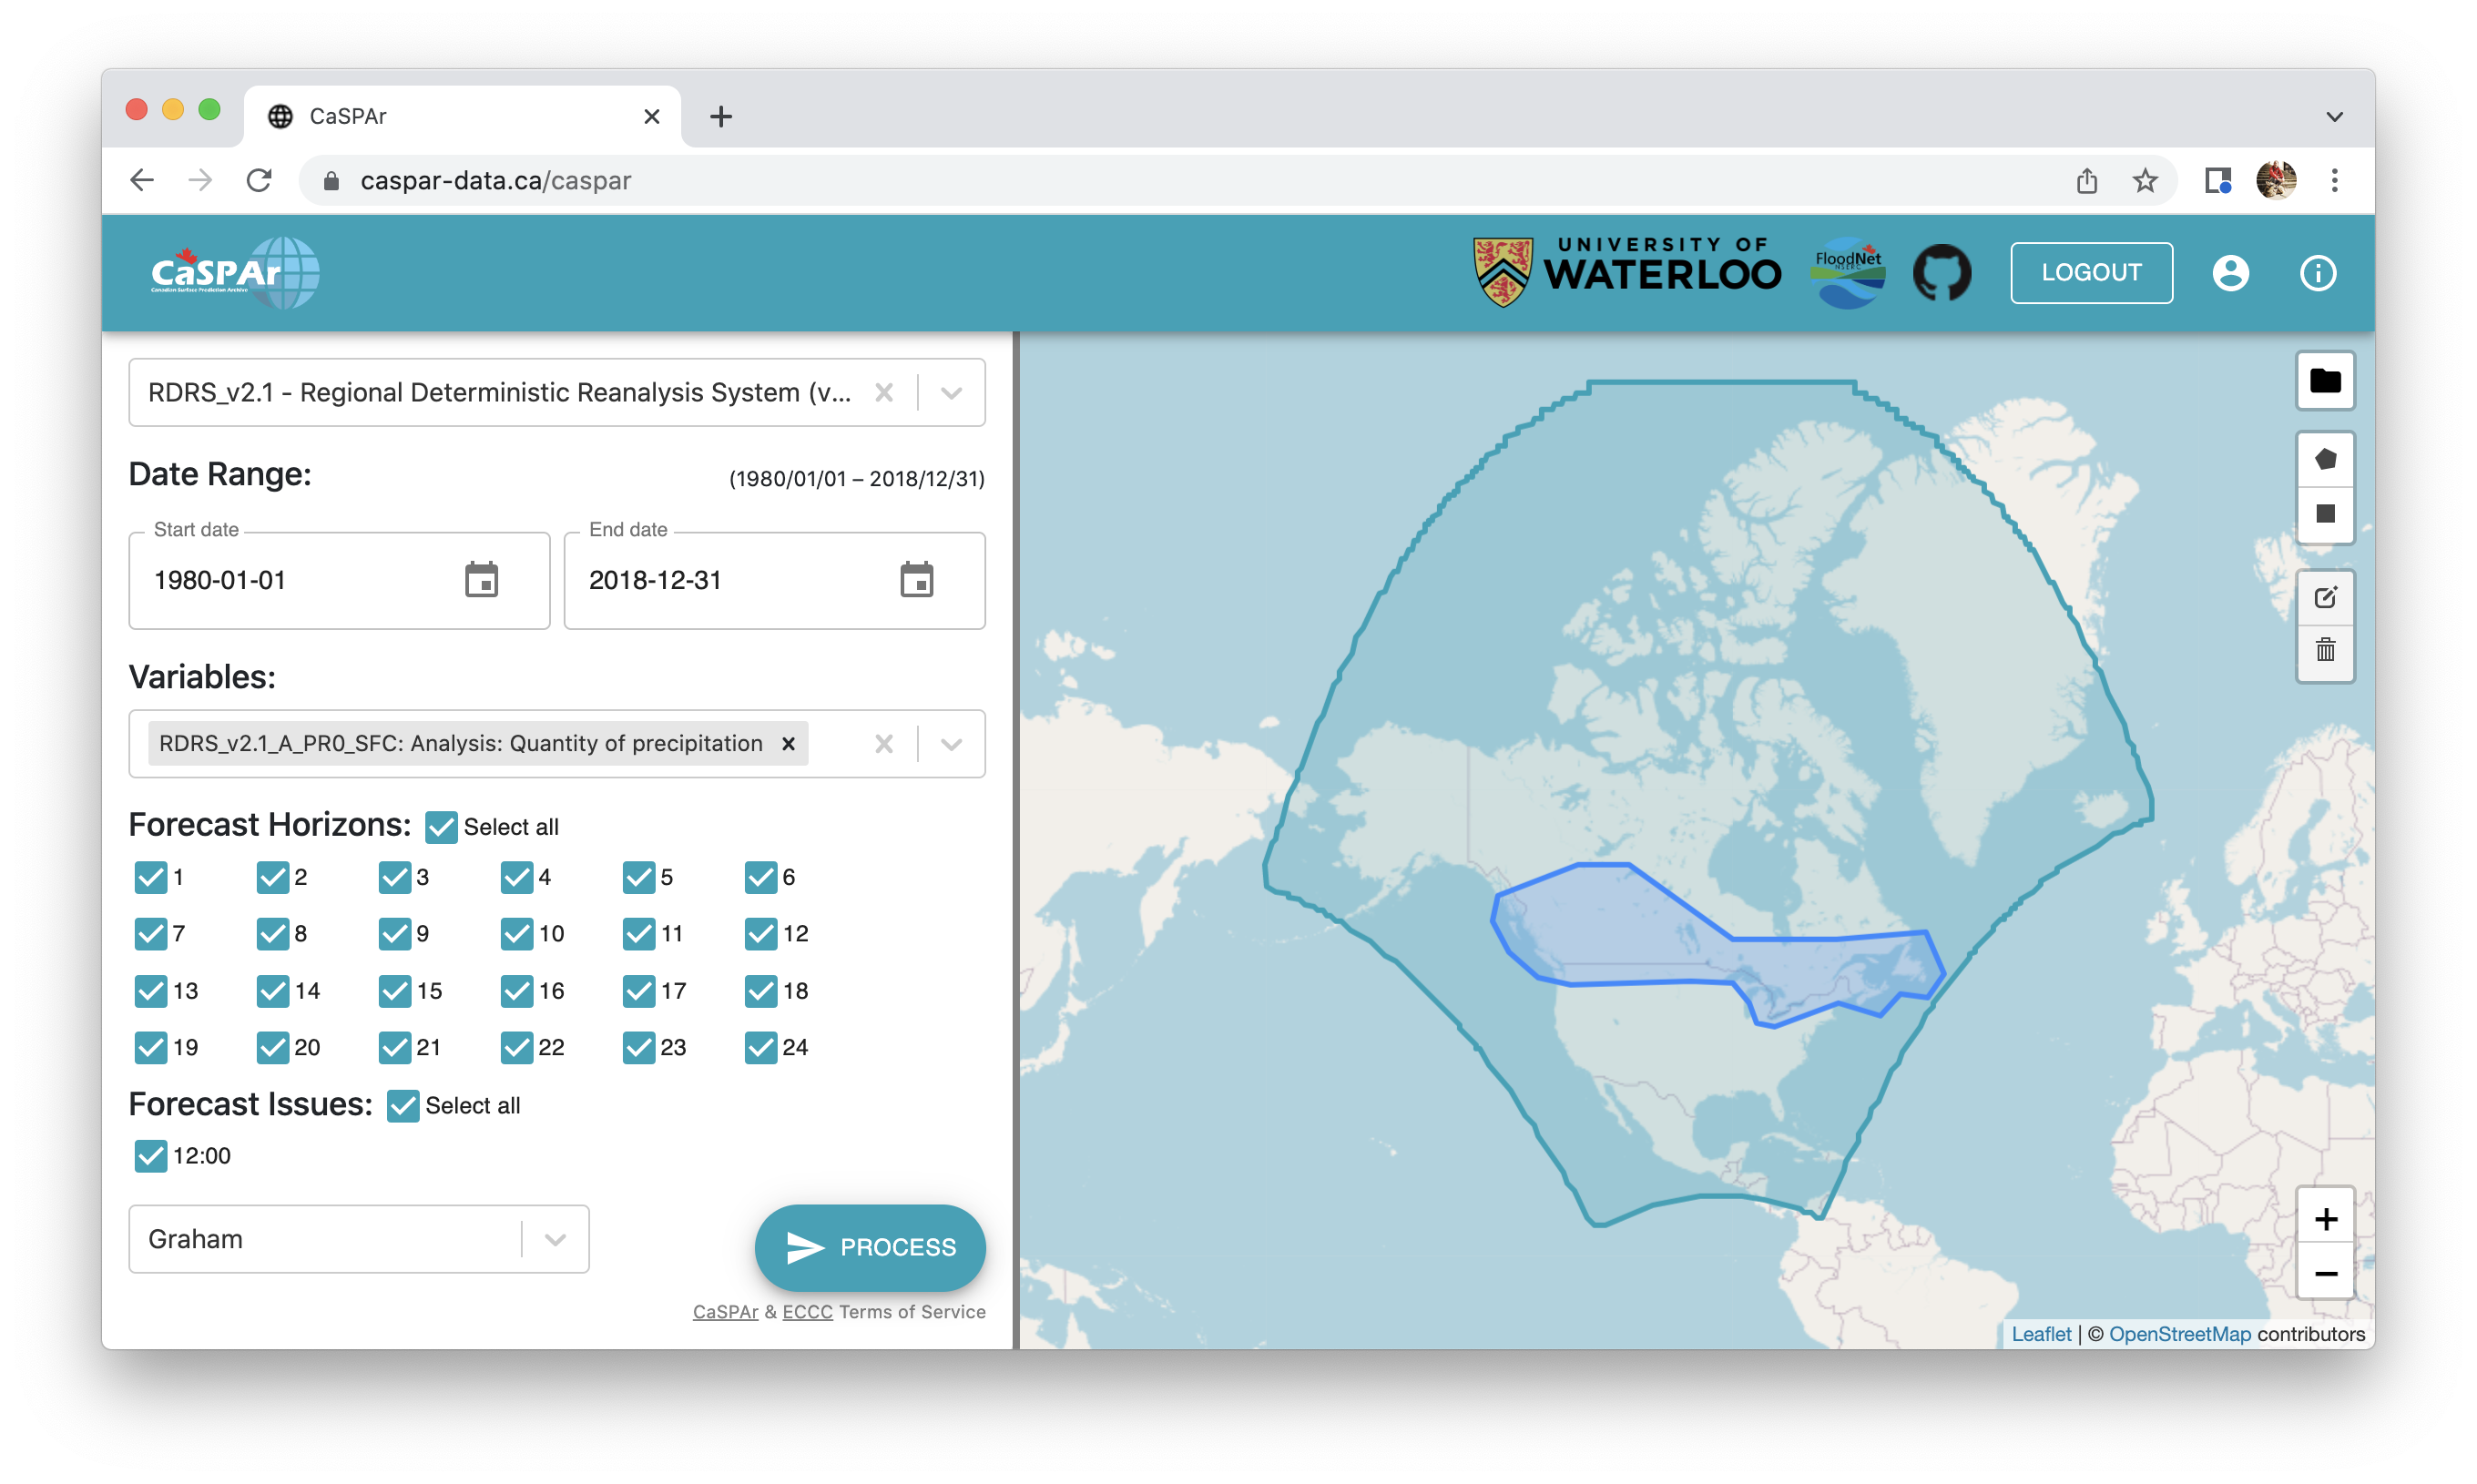
\includegraphics[width=\linewidth]{figures/caspar-request-hfe.png}
	\caption{Screenshot of CaSPAr (\url{https://caspar-data.ca/caspar}) frontend displaying setting to request RDRS-v2.1 for the HFE domain. The shapefile used to define the domain (blue highlighted area) within the data available for RDRS-v2.1 (turquoises highlighted area) is available under \texttt{data/caspar/RDRS\_v21\_hfe\_outline.zip} and has been used via file upload (top button in right top corner of the map).}
	\label{fig:request_data_caspar}
\end{figure}
\pagebreak

\textbf{Step B2:} Read data from CaSPAr files.
\begin{framed}
	\vspace*{-1.2cm}
	\begin{ttfont}
		\begin{tabbing}
			\hspace{1.0cm} \= \hspace{5.2cm} \= \kill \\[4pt]
			\GRAU{\# see module for detailed documentation and example}\\
			from b2\_read\_caspar\_nc import read\_caspar\_nc\\
			\\
			data\_caspar = read\_caspar\_nc(\\
			\> \GRAU{\# Mandatory arguments:}\\
			\> variable=\textit{variable}, \> \GRAU{\# name of variable in CaSPAr}\\
			\> filenames=\textit{filenames}, \> \GRAU{\# dictionary specifying filename per time}\\
			\>  \> \GRAU{\# step, e.g.,}\\
			\>  \> \GRAU{\#  \{ date\_1: [ filename\_1, filename\_2 ],}\\
			\>  \> \GRAU{\# \hspace*{0.2cm}    date\_2: [ filename\_2 ],}\\
			\>  \> \GRAU{\# \hspace*{0.2cm}    date\_3: [ ], ... \}}\\
			\>  \> \GRAU{\# $\curvearrowright$ output of "request\_caspar\_nc()"}\\
			\> \GRAU{\# Optional arguments:}\\
			\> bbox=\textit{bbox}, \> \GRAU{\# dictionary specifying bounding box}\\
			\> lintransform=\textit{lintransform}, \> \GRAU{\# dictionary to specify linear transform of}\\
			\>  \> \GRAU{\# data, e.g., to allow for unit conversions}\\
			\> silent=\textit{silent}, \> \GRAU{\# True for no printing on screen}\\
			\> ) \> 
		\end{tabbing}
	\end{ttfont}
	\vspace*{-0.3cm}
\end{framed}
\vspace*{-0.3cm}
The returned variable \texttt{data\_caspar} is a dictionary that will contain the attributes \texttt{time}, \texttt{lat}, \texttt{lon}, and \texttt{var}. The latter will be 3-dimensional (time, lat, lon). The latitude and longitudes of the files are checked for consistency. The time steps returned are only the time steps where data was available.

\textbf{Step Cx:} Plot data.

Since the data \texttt{data\_caspar} have the same structure as the data read from Geomet (i.e., \texttt{data\_geomet}) the plotting of the data is now exactly the same. See \textbf{Step Cx} above. 

\begin{framed}
	\vspace*{-1.2cm}
	\begin{ttfont}
		\begin{tabbing}
			\hspace{1.0cm} \= \hspace{5.2cm} \= \kill \\[4pt]
			\GRAU{\# see module for detailed documentation and example}\\
			from cx\_plot\_data import plot\_data\\
			\\
			plot\_caspar = plot\_data(\\
			\> \GRAU{\# Mandatory arguments:}\\
			\> var=data\_caspar["var"], \> \GRAU{\# 2D/3D array of values for variable}\\
			\> lat=data\_caspar["lat"], \> \GRAU{\# 2D array of latitudes}\\
			\> lon=data\_caspar["lon"], \> \GRAU{\# 2D array of longitudes}\\
			\> ... \> \GRAU{\# see above "Step Cx" for more arguments }\\
			\> ) \> 
		\end{tabbing}
	\end{ttfont}
	\vspace*{-0.3cm}
\end{framed}
\vspace*{-0.3cm}
The returned variable \texttt{plot\_caspar} is a dictionary that will contain the attributes \texttt{png}, \texttt{gif}, and \texttt{legend}. Each of them are assigned list of the according files created. If no file was created (e.g., no legend), the respective list will be empty.

Fig.~\ref{fig:plot_example:caspar} shows the result of a plot of precipitation (\texttt{RDRS-v2.1\_A\_PR0\_SFC}) in the RDRS-v2.1 product for a domain around Montreal on Aug 9, 2018 at 7:00 am (UTC). For comparison, the other two panels in this figure (i.e., Fig.~\ref{fig:plot_example:api-weather:24h} and Fig.~\ref{fig:plot_example:api-weather:6h}) show the results of plotting data requested from Geomet for the same day but as 24-h and 6-h precipitation accumulations of the RDPA product.

\begin{figure}[h!]
	\begin{subfigure}[a]{0.5\textwidth}
		\centering
		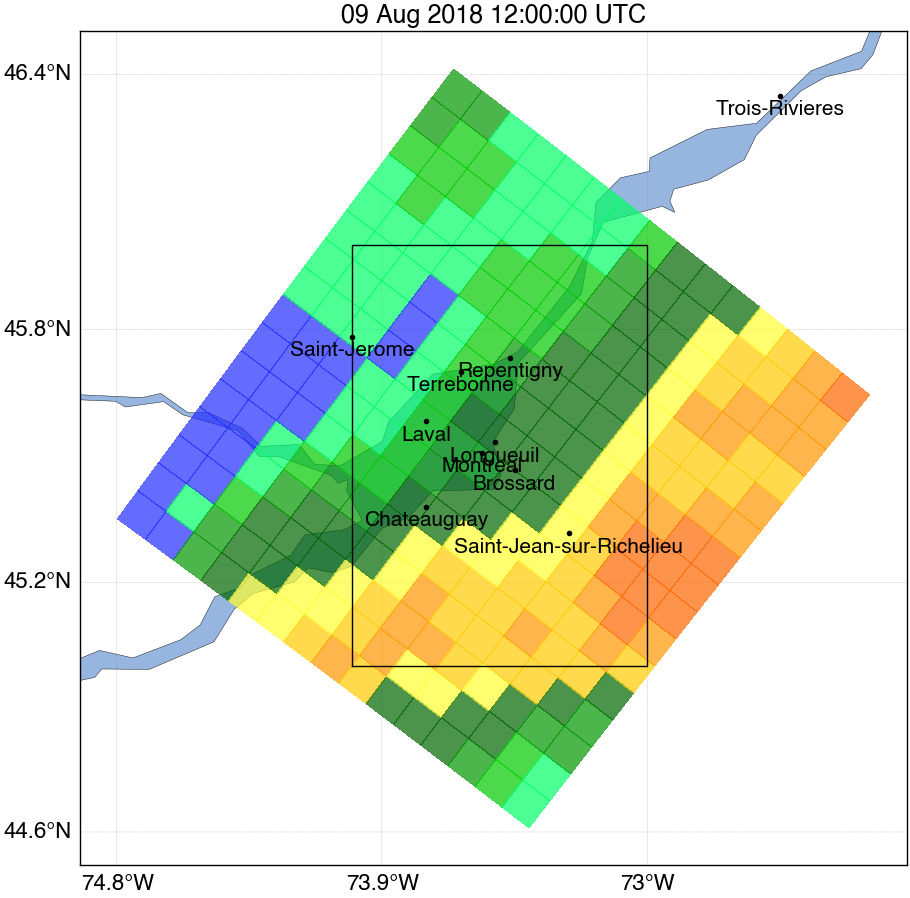
\includegraphics[height=6cm]{figures/test-map-geomet-nrcan-hfe-rdpa24_2018080912.png}
		\caption{PNG produced using NRCan-HFE library based on GRIB2 data (RDPA-24h) retrieved using \url{https://api.weather.gc.ca/}}
		\label{fig:plot_example:api-weather:24h}
	\end{subfigure}
	\hspace*{0.02\textwidth}
	\begin{subfigure}[a]{0.5\textwidth}
		\centering
		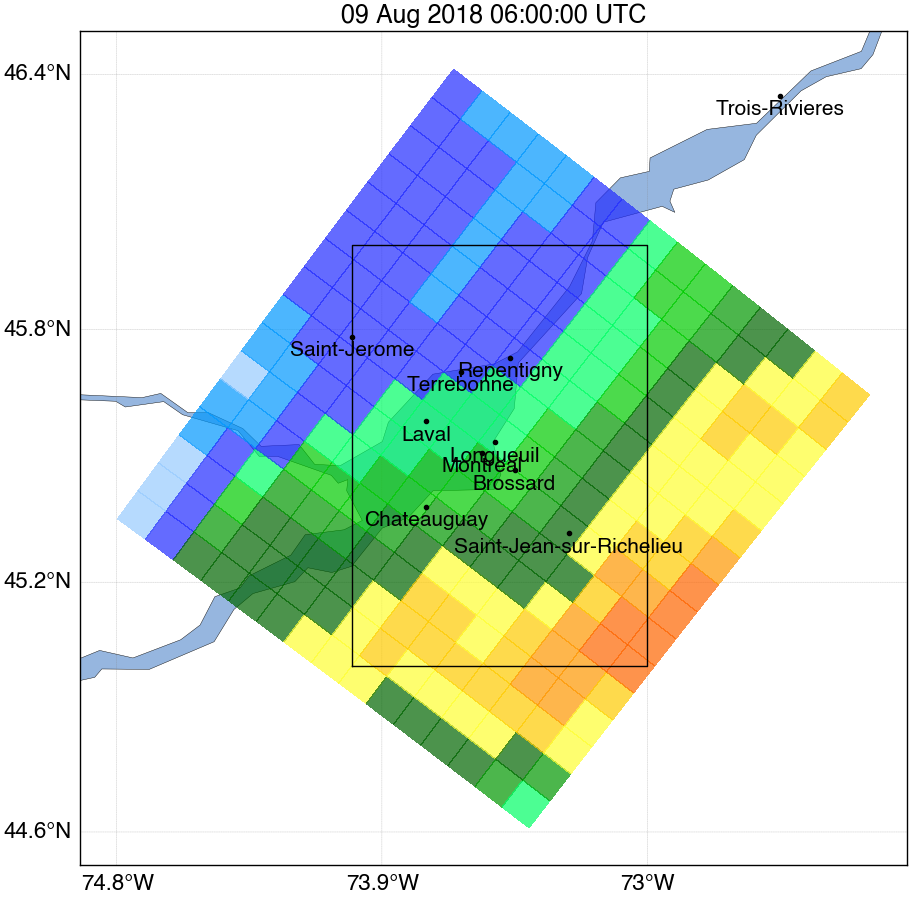
\includegraphics[height=6cm]{figures/test-map-geomet-nrcan-hfe-rdpa6_2018080906.png}
		\caption{PNG produced using NRCan-HFE library based on GRIB2 data (RDPA-6h) retrieved using \url{https://api.weather.gc.ca/}}
		\label{fig:plot_example:api-weather:6h}
	\end{subfigure}\\
	%\hspace*{0.02\textwidth}
	\begin{subfigure}[a]{0.5\textwidth}
		\centering
		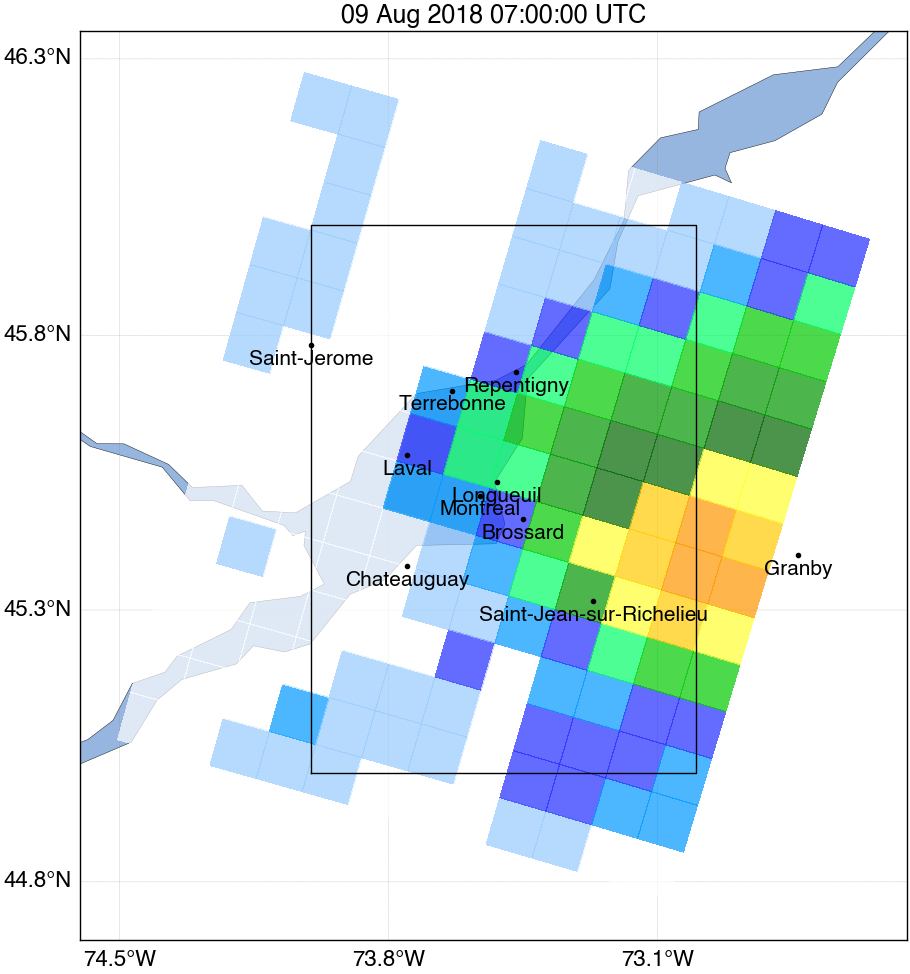
\includegraphics[height=6cm]{figures/test-map-caspar-nrcan-hfe_2018080907.png}
		\caption{PNG produced using NRCan-HFE library based on NetCDF data (RDRS v2.1-1h) retrieved using \url{https://caspar-data.ca}}
		\label{fig:plot_example:caspar}
	\end{subfigure}
	\hspace*{0.02\textwidth}
	\begin{subfigure}[a]{0.5\textwidth}
		\centering
		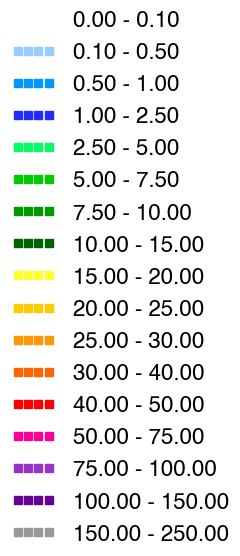
\includegraphics[height=5.2cm]{figures/test-map-caspar-nrcan-hfe_legend.png}
		\caption{Legend for all plots generated.}
		\label{fig:plot_example:legend}
	\end{subfigure}
	\caption{RDPA (24h and 6h total precipitation) from Geomet and RDRS\_v2.1\_A\_PR0\_SFC (1h accumulations) from CaSPAr for data available for Aug 9, 2018. (a) RDPA-24h is accumulated precipitation for noon Aug 8, 2018 (UTC) until noon Aug 9, 2018 (UTC), (b) RDPA-6h is accumulated precipitation for midnight Aug 9, 2018 (UTC) until 6am Aug 9, 2018 (UTC) while (c) RDRS-v2.1 is precipitation between Aug 9, 2018 6:00 am and 7:00 am (UTC). The same bounding box around Montreal has been requested from the three products. (d) The legend is the same for all plots. The panel in Fig.~\ref{fig:plot_example:api-weather:24h} is the same as panel in Fig.~\ref{fig:plot_example:api-weather}. }
	\label{fig:plot_example_geomet-nrcan-hfe_vs_caspar-nrcan-hfe}
\end{figure}
\clearpage

\section{Request and read data from HFE database} 

\textbf{Step A3:} Request HFE database.

The database is available \href{https://open.canada.ca/data/en/dataset/fe83a604-aa5a-4e46-903c-685f8b0cc33c}{here}. It has a web map service (WMS) that can be used to retrieve a GeoJSON containing information about flood events.

However, the database in JSON format was provided by Philippe Aussant on Aug 29, 2022. The data are available under \texttt{data/hfe/}. 

The following data were provided:
\begin{description}
	\item[\texttt{historical\_flood.json \ldots}] This layer contains individual flood
	occurrences (\texttt{points}). The points in this layer have a unique ID
	(\texttt{uuid}) and a secondary key to their historical\_flood\_events
	(\texttt{event\_id}). We need precipitation for these points. You can
	write the precipitation for each in the \texttt{rainfall\_mm}
	attribute. The maps produced in 2.4.1 of SOW are for these points.
	\item[\texttt{historical\_flood\_event.json \ldots}] This layer contains the same
	flood occurrences as the previous layer but now they are grouped
	into events (\texttt{multipoints}). A flood event contains one or more
	occurrence. The unique id of this layer is \texttt{event\_id}. The maps
	produced in 2.4.2 and 2.4.3 of SOW are for these multipoints.
%	\item[\texttt{large\_historical\_flood\_event\_sample.json \ldots}] As discussed in the
%	kickoff meeting, this file contains a sample of the
%	\texttt{historical\_flood\_event} layer. It has three large flood events
%	that contain multiple flood occurrence.
%	\item[\texttt{small\_historical\_flood\_event\_sample.json \ldots}] As discussed in the
%	kickoff meeting, this file contains a sample of the
%	\texttt{historical\_flood\_event} layer. It has three small flood events
%	that contain only one occurrence.
\end{description}

The two files above were used to create some test data under \texttt{src/test-data}. The first few features of each file was taken to create the sample files.

The following function is currently only checking if the files exist at the indicated location, i.e. checking for the existence of the two files \texttt{\textless{}jsonfilebase\textgreater{}.json} and \texttt{\textless{}jsonfilebase\textgreater{}\_event.json}. It is highly recommended that this function is adjusted by NRCan to replicate the formatting of the original data found on the website into these JSON files.

\begin{framed}
	\vspace*{-1.2cm}
	\begin{ttfont}
		\begin{tabbing}
			\hspace{1.0cm} \= \hspace{5.2cm} \= \kill \\[4pt]
			\GRAU{\# see module for detailed documentation and example}\\
			from a3\_request\_hfe\_json import request\_hfe\_json\\
			\\
			files\_hfe = request\_hfe\_json( \\
			\> \GRAU{\# Mandatory arguments:}\\
			\> filename=\textit{filename}, \> \GRAU{\# filename of HFE database (currently not used)}\\
			\> jsonfilebase=\textit{jsonfilebase}, \> \GRAU{\# basename (w/o file ending) of JSON files that }\\
			\> \> \GRAU{\# will be produced (currently just checked for }\\
			\> \> \GRAU{\# existence). Can include path.}\\
			\> \GRAU{\# Optional arguments:}\\
			\> silent=\textit{silent}, \> \GRAU{\# True for no printing on screen}\\
			) \> 
		\end{tabbing}
	\end{ttfont}
	\vspace*{-0.3cm}
\end{framed}
\vspace*{-0.3cm}
The returned variable \texttt{files\_hfe} is a dictionary with one key (\texttt{json}) containing the list of JSON files created (currently just found; not created).
\clearpage

\textbf{Step B3:} Read data from HFE files.
\begin{framed}
	\vspace*{-1.2cm}
	\begin{ttfont}
		\begin{tabbing}
			\hspace{1.0cm} \= \hspace{5.9cm} \= \kill \\[4pt]
			\GRAU{\# see module for detailed documentation and example}\\
			from b3\_read\_hfe\_json import read\_hfe\_json\\
			\\
			data\_hfe = read\_hfe\_json(\\
			\> \GRAU{\# Mandatory arguments:}\\
			\> filename=\textit{filename}, \> \GRAU{\# Name of JSON file of HFE database to read} \\
			\> \GRAU{\# Optional arguments:}\\
			\> filtering=\textit{filtering}, \> \GRAU{\# if True, content of JSON will be checked}\\
			\> \> \GRAU{\# to be consistent and filtered dataset }\\
			\> \> \GRAU{\# returned; checks applied are listed below}\\
			\> polygon=\textit{polygon}, \> \GRAU{\# list of coordinates (lon,lat) of polygon;}\\
			\> \> \GRAU{\# if specified and filtering is}\\
			\> \> \GRAU{\# True, coordinates in JSON are located}\\
			\> \> \GRAU{\# inside this polygon}\\
			\> return\_filtered=\textit{return\_filtered}, \> \GRAU{\# if True, a dictionary will be returned }\\
			\> \> \GRAU{\# listing features that were discarded  }\\
			\> \> \GRAU{\# and reason they were filtered; }\\
			\> \> \GRAU{\# filtered = \{reason: list of feature IDs\}}\\
			\> silent=\textit{silent}, \> \GRAU{\# True for no printing on screen}\\
			\> ) \> 
		\end{tabbing}
	\end{ttfont}
	\vspace*{-0.3cm}
\end{framed}
\vspace*{-0.3cm}
The returned variable \texttt{data\_hfe} is a dictionary that will contain the attributes \texttt{data} and \texttt{filtered}. The latter will be an empty list if \texttt{return\_filtered} is False. Filtering will only be applied if \texttt{filtering} is set to True which is highly recommended. Otherwise, the \texttt{data} are all features found in the JSON file and there is no guarantee that processing using these data will be successful. 

The checks currently applied when \texttt{filtering} is set to True are:
\begin{enumerate}[Check \#1.] 
	\item Required keys are available.
	\item Start and end dates specified are in format YYYY-MM-DD (not just MM or YYYY, etc.).
	\item Start date is 1980-01-01 or later. This is the date RDRS-v2.1 becomes available. For events before this date, no data could be retrieved.
	\item Start date is not before end date (given that end date is specified).
	\item Points and multipoints are within the specified \texttt{polygon} if specified.
\end{enumerate}

Table~\ref{tab:HFE_JSON_feautues} shows the number of features available in the files provided. Different levels of checks are applied, i.e., (i) no checking, (ii) checking everything but not location of coordinates within a polygon (check \#1 to \#3 but not \#4), and (iii) all checks including the test that the features are located within the specified polygon (checks \#1 to \#4). The polygon is set to the extent used to request the CaSPAr data (see \texttt{data/caspar/RDRS\_v21\_hfe\_outline.zip}). Fig.~\ref{fig:plot_example:location_points} shows the location of all events and occurrences as well as the polygon specifying the domain of interest for CaSPAr.

\begin{table}
\begin{tabular}{L{1cm}L{3cm}R{3cm}R{3cm}R{3cm}}
	\hline
	&&  no check & check 1-4 & check 1-5 \\
	&&  \texttt{filtering=False} & \texttt{filtering=True} & \texttt{filtering=True} \\
	&&                           & \texttt{polygon=None}   & \texttt{polygon=polygon} \\
	\hline
	\multicolumn{2}{l}{historical\_flood.json} & 1904 & 1854$^\mathrm{a}$ & 1854$^\mathrm{c}$ \\
	\multicolumn{2}{l}{historical\_flood\_event.json} & 487 & 363$^\mathrm{b}$ & 363$^\mathrm{c}$\\
	\hline
	\multicolumn{1}{r}{$^\mathrm{a}$ $\ldots$} & \multicolumn{4}{l}{in total, n=50 features are flagged;}\\
	& \multicolumn{4}{l}{$\curvearrowright$ n=11 due to check \#2 (only year but not date specified)}\\
	& \multicolumn{4}{l}{$\curvearrowright$ n=39 due to check \#4 (start-date after end-date)}\\
	\multicolumn{1}{r}{$^\mathrm{b}$ $\ldots$} & \multicolumn{4}{l}{in total, n=124 features are flagged; }\\
	& \multicolumn{4}{l}{$\curvearrowright$ n=9 due to check \#2 (only year but not date specified)}\\
	& \multicolumn{4}{l}{$\curvearrowright$ n=110 due to check \#3 (event being before Jan 1, 1980)}\\
	& \multicolumn{4}{l}{$\curvearrowright$ n=5 due to check \#4 (start-date after end-date)}\\
	\multicolumn{1}{r}{$^\mathrm{c}$ $\ldots$} & \multicolumn{4}{l}{in total, n=0 features are flagged due to check \#4}\\
	& \multicolumn{4}{l}{$\curvearrowright$ i.e., all features are inside polygon}\\
	& \multicolumn{4}{l}{$\curvearrowright$ i.e., polygon used to request data from CaSPAr was large enough to cover all events}
\end{tabular}
\caption{Features available in the HFE JSON files provided. Different degrees of filtering show how many features are not conform with requirements to extract precipitation data.}
\label{tab:HFE_JSON_feautues}
\end{table}

\begin{figure}
	\centering
	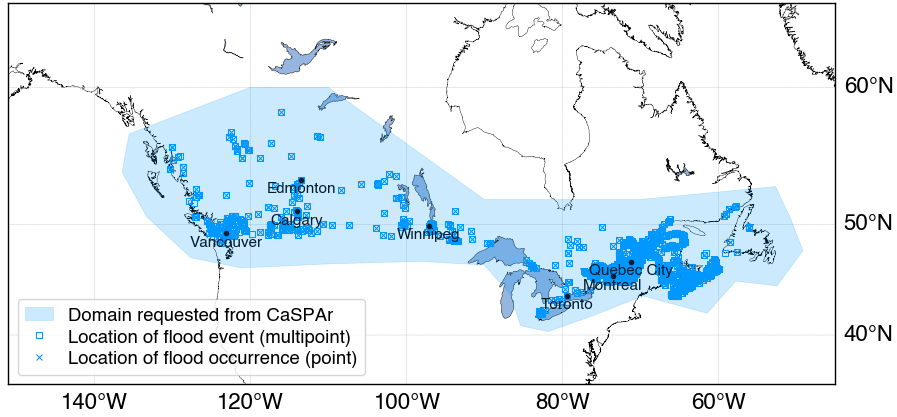
\includegraphics[width=0.8\linewidth]{figures/test-all-coordinates-in-hfe.png}
	\caption{Locations specified in HFE database as multi-point events (squares) or single-point occurrences (crosses) as well as the domain (blue polygon) used to request RDRS-v2.1 from CaSPAr.}
	\label{fig:plot_example:location_points}
\end{figure}

\clearpage

\section{Bilinear interpolation}

\textbf{Step Dx:} a~--~Interpolate data to specific location.

This method is used to extract time series for points defining the flooding event (located within the bounding box used to request data). The raster is interpolated at the flooding event points using bilinear interpolation. The base of this function is \texttt{scipy.interpolate.LinearNDInterpolator} (function \texttt{scipy.interpolate.interp2d} was tested but turned out to be too unstable). If a location is requested that is not available in data, an error is raised. It is recommended to set \texttt{post\_process} to True which will round negative interpolated (precipitation) data to zero unless they are ``too negative''. The latter will raise an error indicating that the interpolation does not seem to work properly.

\begin{framed}
	\vspace*{-1.2cm}
	\begin{ttfont}
		\begin{tabbing}
			\hspace{1.0cm} \= \hspace{4.7cm} \= \kill \\[4pt]
			\GRAU{\# see module for detailed documentation and example}\\
			from dx\_interpolate\_data import interpolate\_data\\
			\\
			interpolated\_points = interpolate\_data(\\
			\> \GRAU{\# Mandatory arguments:}\\
			\> var=\textit{var}, \> \GRAU{\# 2D/3D array of values for variable}\\
			\> lat=\textit{lat}, \> \GRAU{\# 2D array of latitudes}\\
			\> lon=\textit{lon}, \> \GRAU{\# 2D array of longitudes}\\
			\> locations=\textit{locations}, \> \GRAU{\# dict containing "lat" as list of latitudes}\\
			\> \> \GRAU{\# and "lon" as list of longitudes for points }\\
			\> \> \GRAU{\# where field(s) of "var" will be interpolated }\\
			\> \GRAU{\# Optional arguments:}\\
			\> bbox=\textit{bbox}, \> \GRAU{\# if provided locations will be checked to fall}\\
			\> \> \GRAU{\# within; in any case points that are not covered}\\
			\> \> \GRAU{\# by the data will result in an error message of}\\
			\> \> \GRAU{\# the function}\\
			\> return\_tmp=\textit{return\_tmp}, \> \GRAU{\# if True, data and location of the points used}\\
			\> \> \GRAU{\# for interpolation will be returned as dictionary}\\
			\> post\_process=\textit{post\_process}, \> \GRAU{\# if True, negative data will be set to zero;  }\\
			\> \> \GRAU{\# unless they are smaller than -0.1 which will}\\
			\> \> \GRAU{\# raise an error}\\
			\> silent=\textit{silent}, \> \GRAU{\# True for no printing on screen}\\
			\> ) \> 
		\end{tabbing}
	\end{ttfont}
	\vspace*{-0.3cm}
\end{framed}
\vspace*{-0.3cm}
The returned variable \texttt{interpolated\_points} is a dictionary that will contain the attributes \texttt{lat}, \texttt{lon}, and \texttt{var}. The latter will be 2-dimensional with the size of the first dimension being the number of time steps and the size of the second dimension being the number of locations. 

Fig.~\ref{fig:plot_example:bilinear} is showing the result of a bilinear interpolation of two locations over the course of 9 days.
\pagebreak 

\textbf{Step Dx:} b~--~Plot interpolated data.

The module \texttt{dx\_interpolate\_data} also contains a convenience function to plot the interpolated data using \texttt{plot\_interpolated()} similar to what is shown in the left two panels of Fig.~\ref{fig:plot_example:bilinear}. An example output of the function with highlighting some time steps is shown in Fig.~\ref{fig:plot_example:plot_interpolated}.

\begin{framed}
	\vspace*{-1.2cm}
	\begin{ttfont}
		\begin{tabbing}
			\hspace{1.0cm} \= \hspace{7.2cm} \= \kill \\[4pt]
			\GRAU{\# see module for detailed documentation and example}\\
			from dx\_interpolate\_data import plot\_interpolated\\
			\\
			plots\_interpolated = plot\_interpolated(\\
			\> \GRAU{\# Mandatory arguments:}\\
			\> locations=\textit{locations}, \> \GRAU{\# dict containing "lat" as list of }\\
			\> \> \GRAU{\# latitudes and "lon" as list of }\\
			\> \> \GRAU{\# longitudes for points }\\
			\> dates=\textit{dates}, \> \GRAU{\# list of dates "data" are provided for}\\
			\> data=\textit{data}, \> \GRAU{\# dictionary of data containing "lat", }\\
			\> \> \GRAU{\# "lon", and "var" (return of }\\
			\> \> \GRAU{\# "interpolate\_data()")}\\
			\> start\_date\_buffer=\textit{start\_date\_buffer}, \> \GRAU{\# start date incl. buffer}\\
			\> end\_date\_buffer=\textit{end\_date\_buffer}, \> \GRAU{\# end date incl. buffer}\\
			\> pngfile=\textit{pngfile}, \> \GRAU{\# name of PNG file to be created}\\
			\> \GRAU{\# Optional arguments:}\\
			\> highlight\_dates\_idx=\textit{highlight\_dates\_idx}, \> \GRAU{\# indexes of timesteps to highlight}\\
			\> \> \GRAU{\# in plot}\\
			\> start\_date=\textit{start\_date}, \> \GRAU{\# start date listed in HFE database}\\
			\> \> \GRAU{\# (only used to plot vertical line)}\\
			\> end\_date=\textit{end\_date}, \> \GRAU{\# end date listed in HFE database}\\
			\> \> \GRAU{\# (only used to plot vertical line)}\\
			\> label=\textit{label}, \> \GRAU{\# custom label to add below plot}\\
			\> silent=\textit{silent}, \> \GRAU{\# True for no printing on screen}\\
			\> ) \> 
		\end{tabbing}
	\end{ttfont}
	\vspace*{-0.3cm}
\end{framed}
\vspace*{-0.3cm}
The returned variable \texttt{plots\_interpolated} is a dictionary that will contain the key \texttt{"png"} and its value is a list of the PNG file created. 

\begin{figure}[h!]
	\centering
	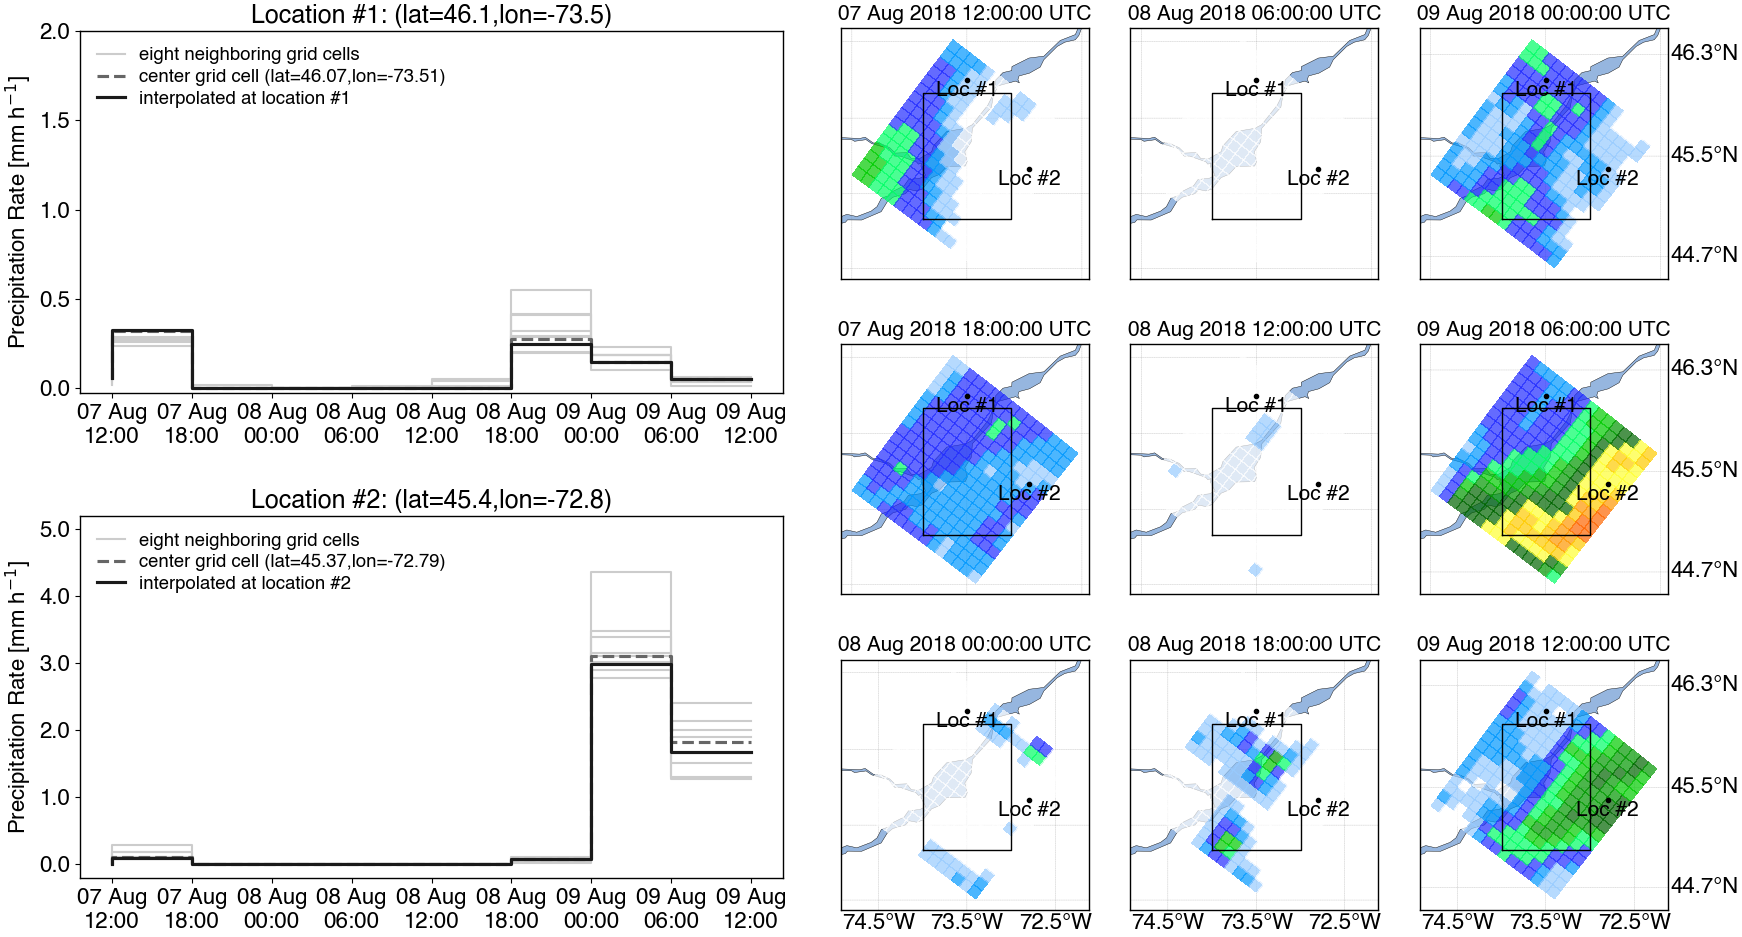
\includegraphics[width=\linewidth]{figures/test-bilinear-interpolation.png}
	\caption{RDPA (6h total precipitation) around Montreal requested from Geomet (\url{https://api.weather.gc.ca/}) is displayed for nine time steps (Aug 7, 2018 12:00 until Aug 9, 2018 12:00). The nine maps on the right show the spatial distribution of precipitation within the requested bounding box (outline of black rectangle) and beyond. The legend is the same for the nine plots showing maps (see Fig.~\ref{fig:plot_example:legend}). Two locations have been randomly selected and are displayed on the maps as well (black dots). The left two panels show the precipitation rate over time for the center cell that contains the locations (dashed black line) as well as the bilinearily interpolated precipitation rate at the exact location (solid black line). For reference also the other 8 neighboring cells used for the bilinear interpolation are shown (gray lines).}
	\label{fig:plot_example:bilinear}
\end{figure}

\begin{figure}[h!]
	\centering
	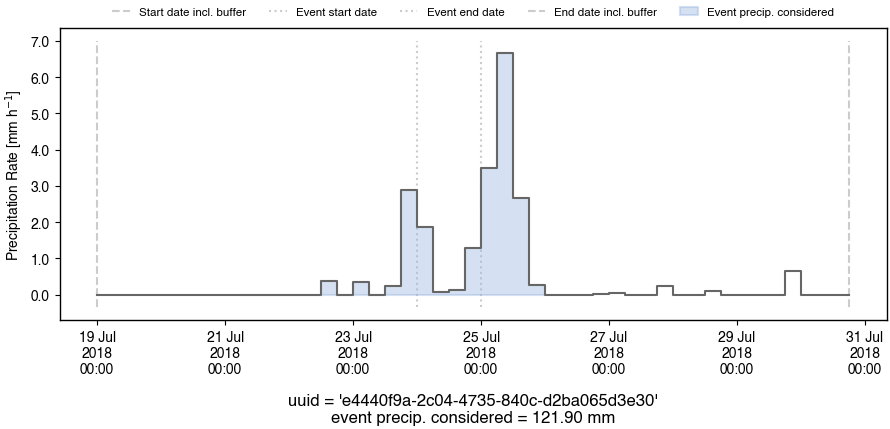
\includegraphics[width=\linewidth]{figures/test-plot-interpolated.png}
	\caption{Output of function \texttt{plot\_interpolated()} in module \texttt{dx\_interpolate\_data}. Some timesteps of the analysed time period from July 19, 2018 to July 31, 2018 have been specified to be highlighted ("\texttt{highlight\_dates\_idx}"; highlighted in blue color). The sum of those datapoints is 121.90 [mm] which had been passed as a custom label ("\texttt{label}") including the UUID of the feature analyzed.}
	\label{fig:plot_example:plot_interpolated}
\end{figure}

\clearpage 

\section{Determine bounding box to process}

\textbf{Step Ex:} Determine bounding box of single-point occurrences or multi-point events.

This function is to determine the bounding box \texttt{bbox} to request data from Geomet and read data retrieved from CaSPAr (see steps A1 and B2, respectively; function argument \texttt{bbox} for both functions). The function is able to handle lists of latitudes and longitudes as well as features directly taken from the HFE database. The features can be single-point occurrences or multi-point events. The bounding box is by default the bounding box around all locations provided with an additional buffer \texttt{bbox\_buffer} of 0.5 degrees in all directions. The buffer can be set to any non-negative value.

\textbf{Note:} The approach might be adjusted/refined once we start processing all flood occurrences and events.

\begin{framed}
	\vspace*{-1.2cm}
	\begin{ttfont}
		\begin{tabbing}
			\hspace{1.0cm} \= \hspace{4.7cm} \= \kill \\[4pt]
			\GRAU{\# see module for detailed documentation and example}\\
			from ex\_determine\_bbox import determine\_bbox\\
			\\
			bbox = determine\_bbox(\\
			\> \GRAU{\# Mandatory arguments:}\\
			\> lat=\textit{lat}, \> \GRAU{\# list of latitude of location(s) that are}\\
			\> \> \GRAU{\# required to be within the bounding box;}\\
			\> \> \GRAU{\# can be scalar if bbox is determined for}\\
			\> \> \GRAU{\# only one location}\\
			\> \> \GRAU{\# either lat/lon \underline{or} feature needs to be specified}\\
			\> lon=\textit{lon}, \> \GRAU{\# list of longitude of location(s) that are}\\
			\> \> \GRAU{\# required to be within the bounding box;}\\
			\> \> \GRAU{\# can be scalar if bbox is determined for}\\
			\> \> \GRAU{\# only one location}\\
			\> \> \GRAU{\# either lat/lon \underline{or} feature needs to be specified}\\
			\> feature=\textit{feature}, \> \GRAU{\# dict containing feature as obtained from}\\
			\> \> \GRAU{\# HFE database;}\\
			\> \> \GRAU{\# either lat/lon \underline{or} feature needs to be specified}\\
			\> \GRAU{\# Optional arguments:}\\
			\> bbox\_buffer=\textit{bbox\_buffer}, \> \GRAU{\# minimum distance between locations provided and}\\
			\> \> \GRAU{\# outline of bounding box (in degrees); needs to}\\
			\> \> \GRAU{\# be non-negative; unit: degree; default 0.5}\\
			\> silent=\textit{silent}, \> \GRAU{\# True for no printing on screen}\\
			\> ) \> 
		\end{tabbing}
	\end{ttfont}
	\vspace*{-0.3cm}
\end{framed}
\vspace*{-0.3cm}
The return value the bounding box in the format of a dictionary which is conform with what is needed for requesting data from Geomet (step A1; \texttt{request\_geomet\_grib2}), read data retrieved from CaSPAr (step B2; \texttt{read\_caspar\_nc}), plotting data (step Cx; \texttt{plot\_data}), and to interpolate data (step Dx; \texttt{interpolate\_data}). 

Fig.~\ref{fig:plot_example:bounding_box} shows the bounding box derived for a single-point occurrence and a multi-point event using different settings for the bounding box buffer \texttt{bbox\_buffer}.

\begin{figure}
	\centering
	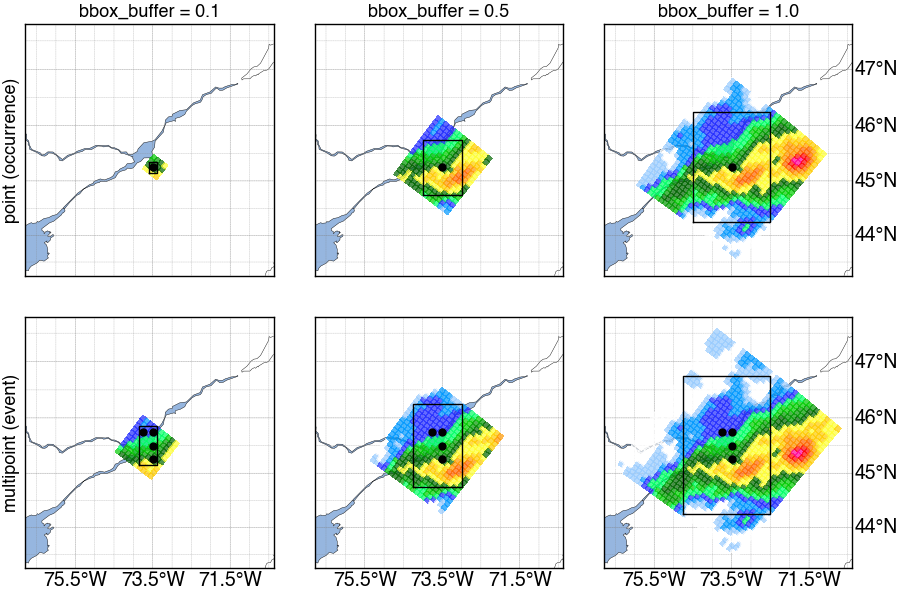
\includegraphics[width=0.7\linewidth]{figures/test-bounding-box.png}
	\caption{Bounding box derived using \texttt{determine\_bbox} using different settings for the buffer between locations and bounding box, i.e., buffer of 0.1 (first column of panels), buffer of 0.5 (second column of panels), and buffer of 1.0 degrees (third column of panels). The results are shown for a single point defining flood occurrences (first row of panels) and multiple points defining flood events (second row).}
	\label{fig:plot_example:bounding_box}
\end{figure}
\clearpage

\section{Determine dates to process}

\textbf{Step Fx:} Determine time steps for single-point occurrences or multi-point events.

This function is to determine all time steps to request data from Geomet and read data retrieved from CaSPAr (see steps A1 and B2, respectively; function argument \texttt{date} for both functions). The function is aware of the timesteps that are available for different products (\texttt{product}) and will return only those valid time steps. A buffer before the specified start date (function argument \texttt{start\_date} or \texttt{feature} property \texttt{start\_date}) and after the specified end date (function argument \texttt{end\_date} or \texttt{feature} property \texttt{end\_date}) is specified via \texttt{dates\_buffer}. The dates are all assumed to be in UTC time. Start dates are assumed to be at 00:00 while end dates are assumed to be at 23:59.

\textbf{Note:} The approach might be adjusted/refined once we start processing all flood occurrences and events.

\begin{framed}
	\vspace*{-1.2cm}
	\begin{ttfont}
		\begin{tabbing}
			\hspace{1.0cm} \= \hspace{4.7cm} \= \kill \\[4pt]
			\GRAU{\# see module for detailed documentation and example}\\
			from fx\_determine\_dates import determine\_dates\\
			\\
			dates = determine\_dates(\\
			\> \GRAU{\# Mandatory arguments:}\\
			\> start\_date=\textit{start\_date}, \> \GRAU{\# start date of event/occurr. as datetime object;}\\
			\> \> \GRAU{\# either start\_date \underline{or} start\_date and end\_date \underline{or}}\\
			\> \> \GRAU{\# feature needs to be specified}\\
			\> end\_date=\textit{end\_date}, \> \GRAU{\# end date of event/occurrence as datetime object;}\\
			\> \> \GRAU{\# if not specified but start\_date is, end\_date will}\\
			\> \> \GRAU{\# be set to start\_date + 1 day;}\\
			\> \> \GRAU{\# either start\_date \underline{or} start\_date and end\_date \underline{or}}\\
			\> \> \GRAU{\# feature needs to be specified}\\
			\> feature=\textit{feature}, \> \GRAU{\# dict containing feature as obtained from}\\
			\> \> \GRAU{\# HFE database; needs to contain feature property }\\
			\> \> \GRAU{\# "start\_date" and "end\_date";}\\
			\> \> \GRAU{\# either start\_date \underline{or} start\_date and end\_date \underline{or}}\\
			\> \> \GRAU{\# feature needs to be specified}\\
			\> product=\textit{product}, \> \GRAU{\# name of product, e.g., "rdpa:10km:24f"}\\
			\> \> \GRAU{\# must be one of the following: }\\
			\> \> \GRAU{\# [ "RDRS\_v2.1", "rdpa:10km:24f", "rdpa:10km:6f" ]}\\
			\> \GRAU{\# Optional arguments:}\\
			\> dates\_buffer=\textit{dates\_buffer}, \> \GRAU{\# used to offset start\_date to}\\
			\> \> \GRAU{\# start\_date - dates\_buffer[0] and end\_date to }\\
			\> \> \GRAU{\# end\_date + dates\_buffer[1] in order to retrieve}\\
			\> \> \GRAU{\# precipitation data prior to and after flooding}\\
			\> \> \GRAU{\# event; needs to be non-negative; unit: days}\\
			\> \> \GRAU{\# default [3.0,1.0]}\\
			\> silent=\textit{silent}, \> \GRAU{\# True for no printing on screen}\\
			\> ) \> 
		\end{tabbing}
	\end{ttfont}
	\vspace*{-0.3cm}
\end{framed}
\vspace*{-0.3cm}
The return value is a list of datetime objects which is conform with what is needed for requesting data from Geomet (step A1; \texttt{request\_geomet\_grib2}), reading data retrieved from CaSPAr (step B2; \texttt{read\_caspar\_nc}), and plotting data (step Cx; \texttt{plot\_data}). The function argument for these three functions is \texttt{date}.
\pagebreak

The following examples are to show the dates determined using this function.

\textbf{Example 1a:} Dates to retrieve data from RDRS\_v2.1 (hourly dataset) without buffer.
\begin{framed}
	\vspace*{-1.2cm}
	\begin{ttfont}
		\begin{tabbing}
			\hspace{1.5cm} \= \hspace{2.7cm} \= \hspace{4.7cm} \= \kill \\[4pt]
			product = "RDRS\_v2.1"\\
			dates\_buffer = [0.0,0.0]\\
			period = [datetime.datetime(2000,5,28,3,0),datetime.datetime(2000,5,29,20,30)]\\
			\\
			\GRAU{\# call function}\\
			tsteps = determine\_dates(start\_date=period[0],end\_date=period[1],\\
			\> \> product=product,dates\_buffer=dates\_buffer)\\
			print(tsteps)\\
			\\
			\GRAU{[Out]: [datetime.datetime(2000, 5, 28, 3, 0),}\\
			\> 	\GRAU{ datetime.datetime(2000, 5, 28, 4, 0), ..., }\\
			\> 	\GRAU{ datetime.datetime(2000, 5, 29, 20, 0) ]   }\\
		\end{tabbing}
	\end{ttfont}
\vspace*{-0.3cm}
\end{framed}
\vspace*{-0.3cm}

\textbf{Example 1b:} Dates to retrieve data from RDRS\_v2.1 (hourly dataset) with buffer.
\begin{framed}
	\vspace*{-1.2cm}
	\begin{ttfont}
		\begin{tabbing}
			\hspace{1.5cm} \= \hspace{2.7cm} \= \hspace{4.7cm} \= \kill \\[4pt]
			product = "RDRS\_v2.1"\\
			dates\_buffer = [3.0,1.0]\\
			period = [datetime.datetime(2000,5,28,3,0),datetime.datetime(2000,5,29,20,30)]\\
			\\
			\GRAU{\# call function}\\
			tsteps = determine\_dates(start\_date=period[0],end\_date=period[1],\\
			\> \> product=product,dates\_buffer=dates\_buffer)\\
			print(tsteps)\\
			\\
			\GRAU{[Out]: [datetime.datetime(2000, 5, 25, 3, 0),}\\
			\> 	\GRAU{ datetime.datetime(2000, 5, 25, 4, 0), ..., }\\
			\> 	\GRAU{ datetime.datetime(2000, 5, 30, 20, 0) ]   }\\
		\end{tabbing}
	\end{ttfont}
	\vspace*{-0.3cm}
\end{framed}
\vspace*{-0.3cm}

\textbf{Example 2a:} Dates to retrieve data from RDPA-6h (6-hourly dataset) without buffer.
\begin{framed}
	\vspace*{-1.2cm}
	\begin{ttfont}
		\begin{tabbing}
			\hspace{1.5cm} \= \hspace{2.7cm} \= \hspace{4.7cm} \= \kill \\[4pt]
			product = "rdpa:10km:6f"\\
			dates\_buffer = [0.0,0.0]\\
			period = [datetime.datetime(2000,5,28,3,0),datetime.datetime(2000,5,29,20,30)]\\
			\\
			\GRAU{\# call function}\\
			tsteps = determine\_dates(start\_date=period[0],end\_date=period[1],\\
			\> \> product=product,dates\_buffer=dates\_buffer)\\
			print(tsteps)\\
			\\
			\GRAU{[Out]: [datetime.datetime(2000, 5, 28, 6, 0),}\\
			\> 	\GRAU{ datetime.datetime(2000, 5, 28, 12, 0), ..., }\\
			\> 	\GRAU{ datetime.datetime(2000, 5, 29, 18, 0) ]   }\\
		\end{tabbing}
	\end{ttfont}
	\vspace*{-0.3cm}
\end{framed}
\vspace*{-0.3cm}

%\textbf{Example 2b:} Dates to retrieve data from RDPA-6h (6-hourly dataset) with buffer.
%
%\textbf{Example 3a:} Dates to retrieve data from RDPA-24h (daily dataset; only available 12:00) without buffer.
%
%\textbf{Example 3b:} Dates to retrieve data from RDPA-24h (daily dataset; only available 12:00) with buffer.

\section{Identify precipitation event}

\textbf{Step Gx:} Identify the major precipitation event in a time series between a specified start and end date as well as shortly before and after.

It is assumed that a precipitation time series is provided (\texttt{"data"}) at given dates (\texttt{"dates"}) for a feature (\texttt{"feature"}) as it is stored in the HFE database. The main event will then be identified starting at the start date given in the
\texttt{"feature"}. A rolling window of a certain length (\texttt{"length\_window\_d"}) will be analyzed. If the accumulated precipitation of the current window is large enough (larger than \texttt{"min\_prec\_window"}), all time steps of the window will be added and the window moved by one timestep (earlier). This is continued until no new time step is added prior to the start date (because the cumulative precipitation is too small, i.e., event start seems to have been found). Then only single time steps (prior to first current index) are checked and added until the first time step smaller than a threshold (\texttt{"min\_prec"}) is detected. This guarantees that the entire onset of the event is added. The same approach is then repeated starting the rolling window with the current
last detected index (current end of event). After no more indexes are added by using the window, single time steps larger
than a threshold (\texttt{"min\_prec"}) are added.

\begin{framed}
	\vspace*{-1.2cm}
	\begin{ttfont}
		\begin{tabbing}
			\hspace{1.0cm} \= \hspace{6.2cm} \= \kill \\[4pt]
			\GRAU{\# see module for detailed documentation and example}\\
			from gx\_identify\_precipitation\_event import identify\_precipitation\_event\\
			\\
			time\_idx = identify\_precipitation\_event(\\
			\> \GRAU{\# Mandatory arguments:}\\
			\> feature=\textit{feature}, \> \GRAU{\# dict containing feature as obtained }\\
			\> \> \GRAU{\# from HFE database}\\
			\> product=\textit{product}, \> \GRAU{\# name of product, e.g., "rdpa:10km:24f"}\\
			\> \> \GRAU{\# must be one of the following: }\\
			\> \> \GRAU{\# [ "RDRS\_v2.1", "rdpa:10km:24f", }\\
			\> \> \GRAU{\# \ \ "rdpa:10km:6f" ]}\\
			\> dates=\textit{dates}, \> \GRAU{\# list of dates "data" are provided for}\\
			\> data=\textit{data}, \> \GRAU{\# dictionary of data containing "lat", }\\
			\> \> \GRAU{\# "lon", and "var" (return of }\\
			\> \> \GRAU{\# "interpolate\_data()")}\\
			\> \GRAU{\# Optional arguments:}\\
			\> length\_window\_d=\textit{length\_window\_d}, \> \GRAU{\# Length of rolling window precipitation }\\
			\> \> \GRAU{\# is iteratively analyzed for.}\\
			\> \> \GRAU{\# Given in [days].}\\
			\> min\_prec\_window=\textit{min\_prec\_window}, \> \GRAU{\# Minimum precipitation accumulated over }\\
			\> \> \GRAU{\# rolling window to be considered being}\\
			\> \> \GRAU{\# added to event. }\\
			\> \> \GRAU{\# Given in [mm] within length\_window\_d.}\\
			\> min\_prec=\textit{min\_prec}, \> \GRAU{\# Minimal amount of precipitation to be  }\\
			\> \> \GRAU{\# considered at one time step.  }\\
			\> \> \GRAU{\# Given in [mm/h].}\\
			\> silent=\textit{silent}, \> \GRAU{\# True for no printing on screen}\\
			\> ) \> 
		\end{tabbing}
	\end{ttfont}
	\vspace*{-0.3cm}
\end{framed}
\vspace*{-0.3cm}
The return value \texttt{"time\_idx"} is a list of list of indexes for time steps that should be considered as major precipitation event. The indexes can be applied to \texttt{"dates"} and the time axis of \texttt{"data"}. The list of list of indexes can be helpful to be specified as \texttt{"highlight\_dates\_idx"} in \texttt{plot\_interpolated()}.

The result of three example events that occurred in 2017 comparing data retrieved from Geomet (RDPA-6h) and CaSPAr (RDRS\_v2.1) are shown in Fig.~\ref{fig:plot_example:prec_event_caspar_vs_geomet}.

\begin{figure}[h]
	\begin{subfigure}[a]{0.48\textwidth}
		\centering
		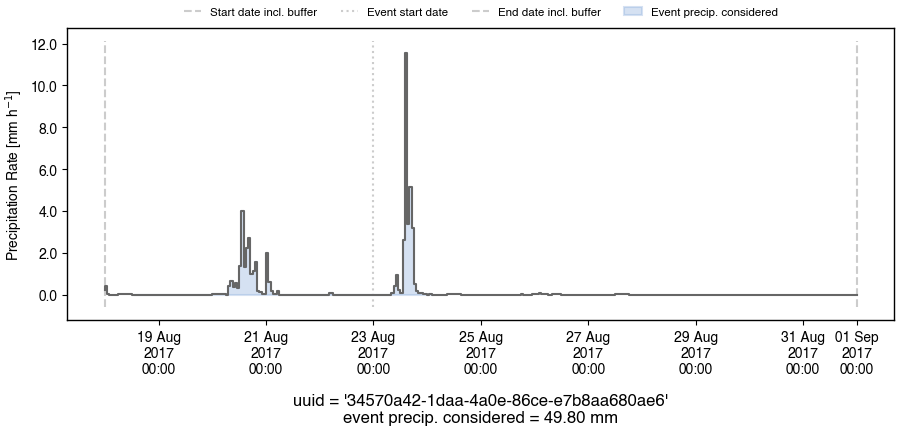
\includegraphics[width=\linewidth]{figures/compare_Geomet_CaSPAr/interpolated_at_stations_occurrence_883_identified-timesteps_RDRS_v2.1.png}
		\caption{UUID ``34570a42-1daa-4a0e-86ce-e7b8aa680ae6''\\using CaSPAr data (RDRS\_v2.1; 1hr accum.)}
	\end{subfigure}
	%\vspace*{0.05\textwidth}
	%\par\bigskip\bigskip
	\hspace*{0.05\linewidth}
	\begin{subfigure}[a]{0.48\textwidth}
		\centering
		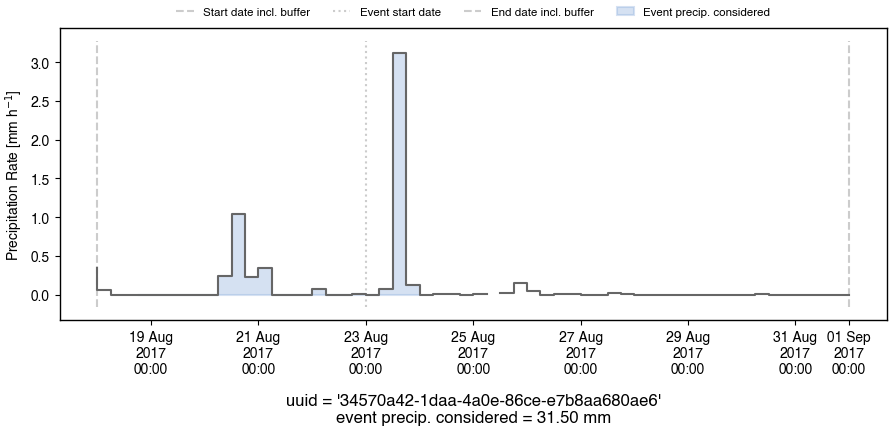
\includegraphics[width=\linewidth]{figures/compare_Geomet_CaSPAr/interpolated_at_stations_occurrence_883_identified-timesteps_rdpa:10km:6f.png}
		\caption{UUID ``34570a42-1daa-4a0e-86ce-e7b8aa680ae6''\\using GeoMet data (RDPA; 6hr accum.)}
	\end{subfigure}
	\par\bigskip\bigskip
	%
	\begin{subfigure}[b]{0.48\textwidth}
		\centering
		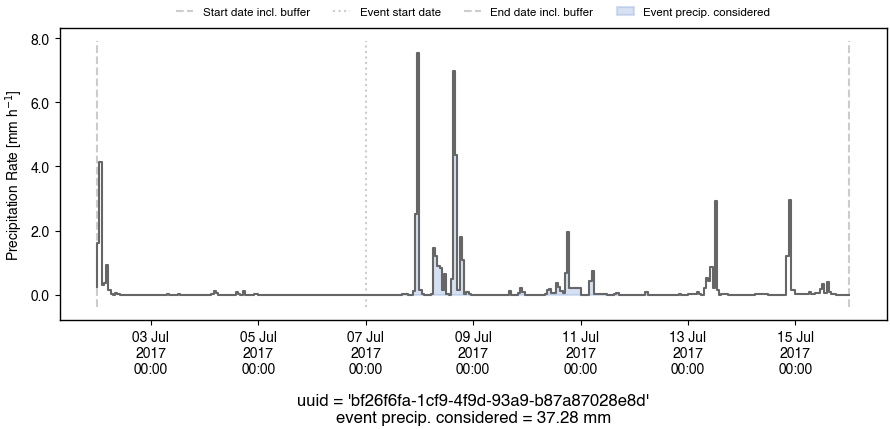
\includegraphics[width=\linewidth]{figures/compare_Geomet_CaSPAr/interpolated_at_stations_occurrence_1362_identified-timesteps_RDRS_v2.1.png}
		\caption{UUID ``bf26f6fa-1cf9-4f9d-93a9-b87a87028e8d''\\using CaSPAr data (RDRS\_v2.1; 1hr accum.)}
	\end{subfigure}
	%\vspace*{0.05\textwidth}
	%\par\bigskip\bigskip
	\hspace*{0.05\linewidth}
	\begin{subfigure}[b]{0.48\textwidth}
		\centering
		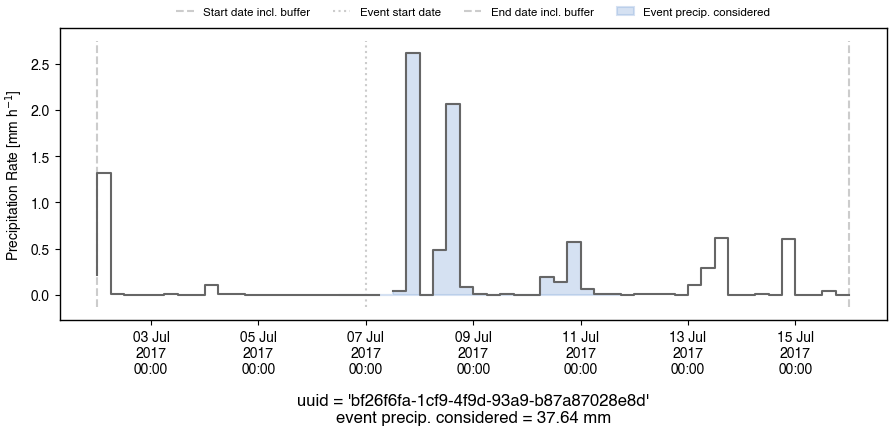
\includegraphics[width=\linewidth]{figures/compare_Geomet_CaSPAr/interpolated_at_stations_occurrence_1362_identified-timesteps_rdpa:10km:6f.png}
		\caption{UUID ``bf26f6fa-1cf9-4f9d-93a9-b87a87028e8d''\\using GeoMet data (RDPA; 6hr accum.)}
	\end{subfigure}
	\par\bigskip\bigskip
	%
	\begin{subfigure}[c]{0.48\textwidth}
		\centering
		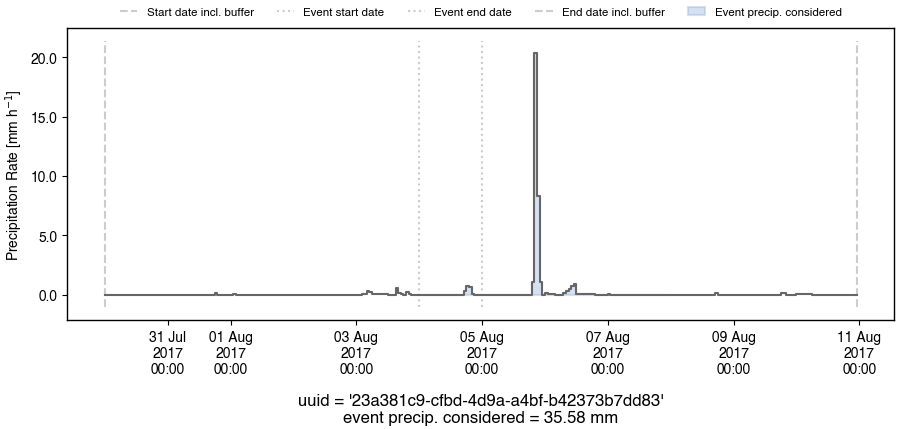
\includegraphics[width=\linewidth]{figures/compare_Geomet_CaSPAr/interpolated_at_stations_occurrence_1756_identified-timesteps_RDRS_v2.1.png}
		\caption{UUID ``23a381c9-cfbd-4d9a-a4bf-b42373b7dd83''\\using CaSPAr data (RDRS\_v2.1; 1hr accum.)}
	\end{subfigure}
	%\vspace*{0.05\textwidth}
	%\par\bigskip\bigskip
	\hspace*{0.05\linewidth}
	\begin{subfigure}[c]{0.48\textwidth}
		\centering
		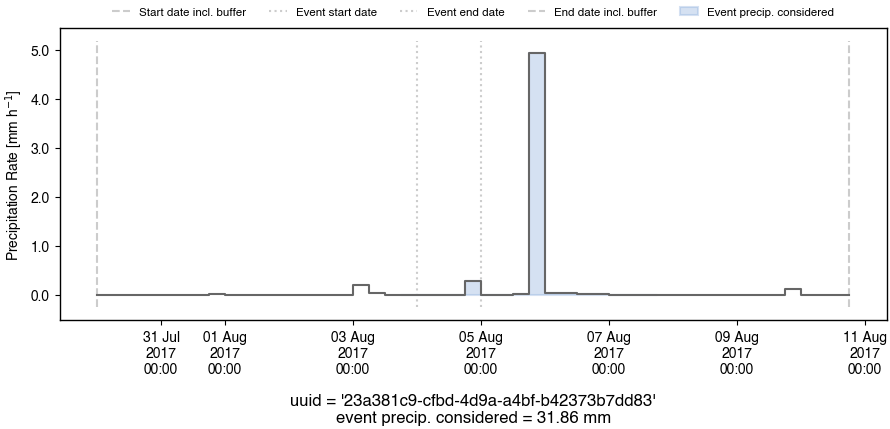
\includegraphics[width=\linewidth]{figures/compare_Geomet_CaSPAr/interpolated_at_stations_occurrence_1756_identified-timesteps_rdpa:10km:6f.png}
		\caption{UUID ``23a381c9-cfbd-4d9a-a4bf-b42373b7dd83''\\using GeoMet data (RDPA; 6hr accum.)}
	\end{subfigure}
	\par\bigskip\bigskip
	\caption{Three example flood events (rows) that occurred in 2017 from HFE database (historical\_flood.json). The major precipitation has been identified using CaSPAr data (left column) and GeoMet data (right column). The identified for each event (UUID) corresponds to the UUID specified in \texttt{historical\_flood.json}.}
	\label{fig:plot_example:prec_event_caspar_vs_geomet}
\end{figure}


\end{document}



